\chapter{Object reconstruction and identification}
\label{Ch:ObjectsDef}
%\minitoc
The format of the raw data collected by the CMS detector is in detector hits and deposited charge information. Therefore, it is not suitable to be used directly in the  analysis.\\
In this chapter, the reconstruction and identification of objects, such as jets, electrons, muons, used in the CMS experiment is discussed.
These objects and their kinematic characteristics are subsequently used for defining the event selection criteria, which will be discussed in Ch.~\ref{Chap:eventSel}.\\
Figure~\ref{fig:CMS_Slice} displays the tracks of the particles as they pass through the sub-detectors of the CMS experiment. Only energy deposits in the most relevant sub-detectors are presented, because a particle can leave trace in multiple detector layers.
The charged particle trajectories (tracks) and origins (vertices) can be determined from the signals (hits) in the tracker layers.
The charged particle trajectories are bent due to the magnetic field and this allows to measure the electric charge and the momentum.
After the tracker, electrons and photons are absorbed in the \acrshort{ecal} and leave their signatures as clusters of energy recorded in adjacent cells. Using this information, energy and direction of the electromagnetically interacting particles can be determined. Charged~(ch.) and neutral hadrons are fully absorbed in the \acrshort{hcal}; however, they may initiate a hadronic shower in the \acrshort{ecal} as well. As in the case of electromagnetically interacting particles, energies and directions of hadrons can be estimated using the corresponding clusters. Muons produce hits in muon detectors which are actually additional trackers located outside the calorimeters.
The only particles known from the \acrshort{sm} and do not leave any trace in the detector are neutrinos.\\
\begin{figure}
\begin{center}
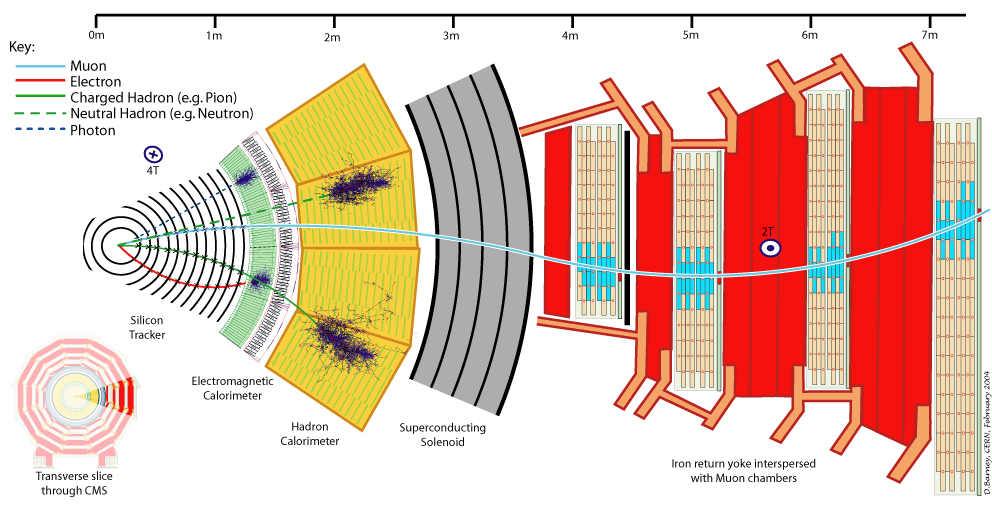
\includegraphics[width=\textwidth]{Plots/CMS/CMS_Slice}
\caption[Cross section of a slice of the CMS detector]{\label{fig:CMS_Slice} Cross section of a slice of the CMS detector in the transverse plane with different particles crossing the subsystems is shown~\cite{CMS_slice}. Only energy deposits in the most relevant subdetectors are presented for simplicity.}
\end{center}
\end{figure}
\section{Particle-Flow algorithm}
\label{sec:PF}
The \acrfull{pf} algorithm~\cite{PF}, uses the information obtained from all of the detector subsystems in the object reconstruction. The three main object collections that feed into the PF algorithm are the tracks reconstructed from hits in the tracker, energy deposits in the calorimeters, and muon candidates reconstructed from hits in the muon system.
In order to achieve object reconstruction with a high efficiency and low fake rate, iterative tracking and the calorimeter clustering methods are used in the PF algorithm.\\
The Kalman filter~\cite{KalmanFilt} method is adopted to determine single particle tracks (See Sec.~\ref{sec:PV}). Calorimeter clustering is responsible for four tasks: the detection and measurement of the energy and the direction of the stable neutral particles, their isolation from charged hadron energy deposits, reconstruction and identification of electrons and all corresponding Bremsstrahlung photons, and help the energy measurement of charged hadrons for which the track parameters were not determined accurately. After determining the single elements, a linking algorithm is used to form a block from separate elements such as tracks, muons, ECAL clusters, HCAL clusters that are possibly related to a single object. After the construction of blocks, the actual particle reconstruction and identification is performed.\\
The PF algorithm proceeds in steps according to the approximate level of ambiguity for each reconstructed objects; it starts with muons, then electrons follow, finally, it produces photons and neutral particle candidates from the remaining calorimeter clusters to arrive at a global event description.
Following to each step, already identified blocks are gradually discarded.\\
For muons, the tracks in the muon system is re-fit including the (inner) tracker track to form "global" muons if the $\chi^2$ is acceptable~\cite{muon7TeV}.
%fit to the inner tracks by requiring an acceptable $\chi^2$. These muons are also called global muons.
If the momentum of a global muon is compatible with the tracker-only measurement within three standard deviations, the muon hypothesis is kept in PF.\\
Electrons emit a bremsstrahlung radiation, which necessitates a complicated reconstruction procedure to properly associate the radiated energy with the electron candidate. The Gaussian sum filter algorithm~(GSF)~\cite{GSF} allows such recovery and is hence used in the electron reconstruction.
%which also accounts for the possible energy loses is used to perform the track fitting. 
%To ensure an optimal energy containment, all ECAL clusters in the PF block linked either to the supercluster or to one of the GSF track tangents are associated with the candidate. 
%Moreover, all ECAL clusters in the PF block linked either to the supercluster or to one of the GSF track tangents are associated with the PF candidate, To ensure an optimal energy containment.
To ensure an optimal energy containment, all ECAL clusters in the PF block, which are linked to the electron GSF track or to the supercluster, are associated with a PF electron candidate if stringent requirements on the compatibility of the track and the cluster are satisfied.\\
%based on ECAL superclusters determines the electromagnetic energy deposits that are aligned to electron candidate tracks. A particle-flow electron is formed, if the track-cluster compatibility is satisfied.\\
Having removed deposits associated with the reconstructed muons and electrons from the list of PF inputs, the neutral and charged hadrons are reconstructed from the remaining tracks. Naturally, for charged hadrons the matching calorimeter clusters are also used in this stage.\\
%Then, the individual PF objects, such as electrons, photons, muons, charged and neutral hadrons, are combined to form more complex objects: jets, or missing transverse energy.\\
%The reconstruction for photons and $\tau$-leptons will not be described since they are not used in this analysis. Detailed description of these objects can be found here \cite{Photon1}. \\
%In this analysis, the kinematic variables, which are introduced in Chapter \ref{Chap:eventSel}, are based on the reconstructed objects satisfying certain identification criteria.
After the PF algorithm, the list of particle candidates (electrons, photons, muons, charged and neutral hadrons) is fed into the higher level algorithms for example jet clustering which are discussed in the following section.\\
In this work, and from now on, all event observables are based on the list of PF candidates as produced by the PF algorithm.
%The particle candidates are reconstructed in a sequence of highest reconstruction performance to lowest, thus already identified blocks are gradually discarded for the more ambiguous object reconstructions. \\
\section{Tracks and primary vertices}
As discussed in Sec.~\ref{lhc_params}, the LHC is designed to run with a peak instantaneous luminosity of $\mathcal{L}=10^{34}\,{\rm cm^{-2}s^{-1}}$ with the proton bunches crossing at intervals of 25~ns. 
In 2016, the peak luminosity measured by the CMS experiment is 15.30~$10^{33}\,{\rm cm^{-2}s^{-1}}$ (see Fig.~\ref{fig:peaklumi_IntLumi}). Figure~\ref{fig:CMSpileup} shows the recorded luminosity with respect to the mean number of interactions per bunch crossing in the 2016 pp run at 13 TeV with $\rm <n_{vertex}>$=27. These multiple interactions are known as pileup. Due to finite time resolution of the detector, pileup is affected by the prior or later bunch crossings as well. Given these conditions, reconstructing tracks and subsequently the primary vertices is challenging~\cite{PV_1}.\\ 
%the CMS tracker is expected to be exposed by about 1000 charged particles at each bunch crossing.
%Given these conditions, the CMS tracker is expected to be traversed by about 1000 charged particles at each bunch crossing.
%Primary vertices are spread over a luminous region which is known as the beam spot. 
The purpose of primary-vertex reconstruction~\cite{PV_2} is to determine the location of all proton-proton interaction vertices in each event and the associated uncertainty on them, including the ‘signal’ vertex and any vertices from pileup collisions. It uses the available reconstructed tracks and consists of three steps.
%selection of the tracks, clustering of the tracks that appear to originate from the same interaction vertex, and fitting for the position of each vertex using its corresponding tracks.\\
The reconstruction commences with selecting a set of tracks based on some quality criteria such as the number of hits in the tracker and the impact parameter. Next, the selected tracks are clustered using a deterministic annealing (DA) algorithm~\cite{PV_3} which is finding the global minimum for a problem with many degrees of freedom. To overcome outliers that  originate from a secondary or mismeasured tracks, the DA algorithm is extended with a rejection term which acts as a cutoff against the outliers. As a result the DA algorithm becomes a one-dimensional robust adaptive multi-vertex fit~\cite{mvf}. After determining candidate vertices with the DA clustering in z, the candidates containing at least two tracks are then re-fitted using an adaptive vertex fitter~\cite{VertFit}. In the adaptive vertex fit, each track in the vertex is assigned a weight from 0 to 1. The tracks get a weight close to 1 when they are consistent with the position of the reconstructed vertex. The number of degrees of freedom:
\begin{equation}
    n_{\rm dof} = -3 + 2 \sum\limits_{i=1}^{\# tracks} w_i ,
\end{equation}
where $w_i$ is the weight for the $i$th track which is associated to a vertex. As a result, the value of $n_{\rm dof}$ is correlated with the number of tracks arising from the interaction region. Therefore, this can be also used to select true proton-proton interactions.\\
Finally, the number of good primary vertices includes vertices consistent with the luminous region (where the collisions happen),which is also known as beam spot, and with a $n_{\rm dof}\geq4$, corresponding to a minimum of four tracks.\\
%according to their z-coordinate. A vertex fit \cite{VertFit} is then applied on the clusters that more than 1cm apart and contain at least two tracks. 
The primary vertex of interest is chosen to be the vertex with the largest sum of the squared track momenta whereas the other vertices are considered as pileup vertices. The pileup vertex reconstruction and identification efficiency is about 70\%~\cite{JME2008}.\\
In the present analysis, at least a good primary vertex is required in the event selection.
\label{sec:PV}
\begin{figure}
\begin{center}
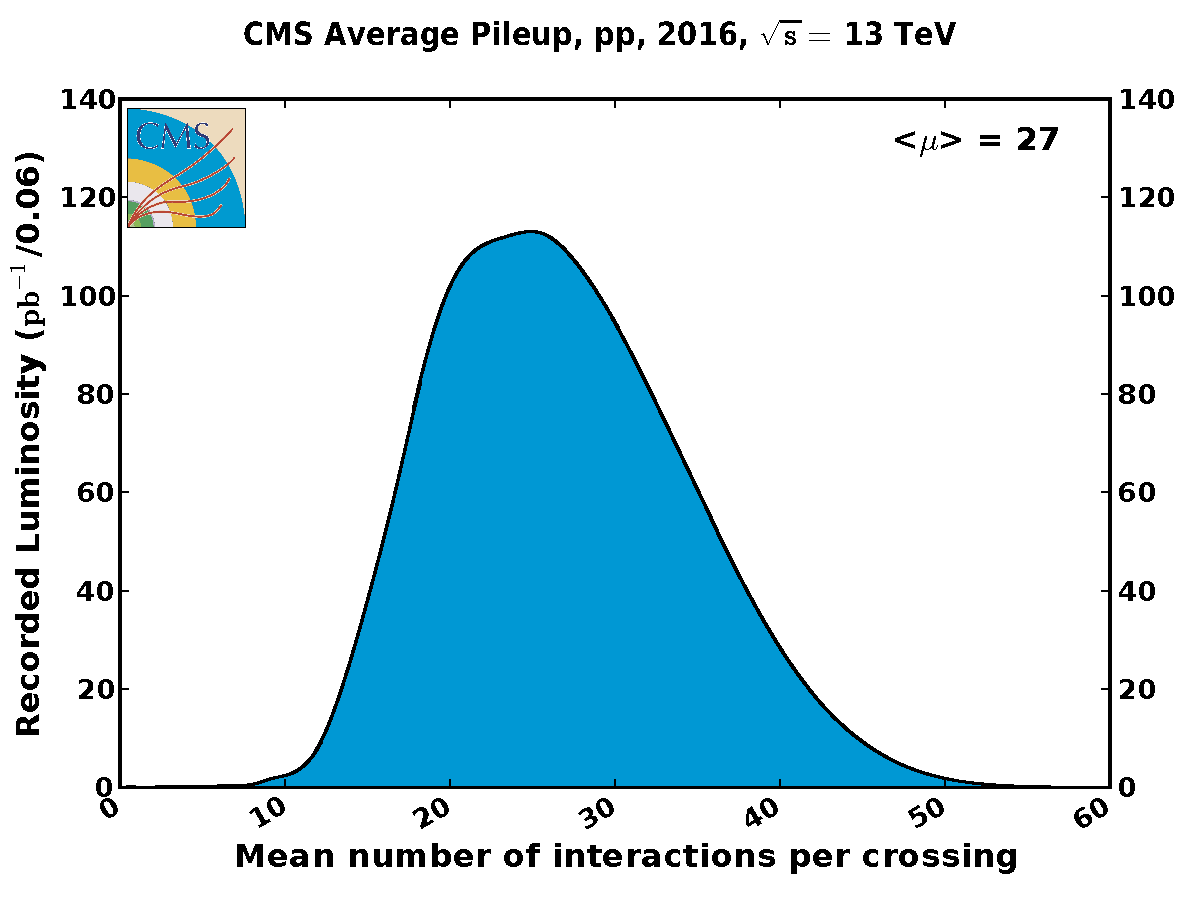
\includegraphics[width=0.8\textwidth]{Plots/CMS/pileup_pp_2016.pdf}
\caption[The mean number of interactions per bunch crossing]{\label{fig:CMSpileup} 
The recorded luminosity of data with respect to the mean number of interactions per bunch crossing in the 2016 pp run at 13~TeV~\cite{pileupCMS}. The cross section is taken to be 80~mb.}
\end{center}
\end{figure}
%%%%%%%%%%%%%%%%
%%%%%%%%%%%%%%%%
\section{Jets}
\label{sec:PFJET}
In the decays of supersymmetric gluinos, an abundance of jets is expected in the final state.\\
As already briefly mentioned in Sec.~\ref{sec:StandardModelParticleInteractions}, cascade decays of quarks and gluons lead to collimated sprays of hadrons that are reconstructed as jets. The main purpose is to reproduce the energy of the original parton prior to the shower. Jets are clustered from all PF candidates using the anti-k$_T$ algorithm~\cite{antiKT}. 
%As jets of particles propagate through the CMS detector, according to their particle content, they leave traces in all of the sub-detectors. To form a reconstructed jet, all these detector responses are combined using various jet algorithms.  
%In CMS there are two types of jet clustering algorithms in use: Cone algorithms and sequential algorithms. The first one uses a geometrical shape assumption, while the latter starts with clustering two of the closest objects together and iteratively reconstruct a closed area of objects until a truncation criterion is satisfied \cite{JET1}.\\
The algorithm starts with clustering two of the closest objects together and iteratively reconstructs a closed area of objects until a truncation criterion is satisfied.
The distance used as the termination criterion can be formulated:
\begin{eqnarray}
{d_{i,\,j} =  min\,(k^{-2}_{{\rm t},i},k^{-2}_{{\rm t},j})\frac{\Delta^2_{i,\,j}}{R^2}}\,,\\
{d_{i,\,B}} = k^{-2}_{{\rm t},i}\,,
\end{eqnarray}
where $d_{i,\,j}$ represents the distance between entities (particles, pseudojets) $i$ and $j$ with R=0.4 and $d_{i,\,B}$ is for the distance between the entity $i$ and the beam ($B$). In the formula, $\Delta^2_{i,\,j}$ is the spatial distance in $y-\phi$ plane and $k_{{\rm t},i}$ is the transverse momentum. The $d_{i,\,j}$ is calculated iteratively until it is $d_{i,\,B}$ and then i is called a jet and it is removed from the list of entities. \\
If the energy fraction of one of the components (e.g. the neutral energy fraction which is dominated by the HCAL subdetector) exceeds 99\% then the jet is rejected, because the probability of a spurious jet from detector noise is high in such cases.\\
%According to different values of $p$, which is governing the relative power of the energy versus geometrical ($\Delta_{i,\,j}$) scales, three main algorithms can be defined.\\
%The case of $p=0$ corresponds to the Cambridge/Aachen algorithm where the termination condition is described by purely geometrical distance. The $p=1$ case is called the ${\rm k_t}$ algorithm which involves the transverse momenta of the entites as well as the geometrical distance parameter. \\
%In this analysis, the anti-${\rm k_t}$ algorithm, which is the case of $p=-1$, is used to cluster the particle flow candidates into jets. For the curious readers, the anti-${\rm k_t}$ algorithm and its performance in comparison to other algorithms are explained here \cite{antiKT}.\\
%In the present search, particle flow candidates are clustered into $R = 0.4$ jets. Jets are required to be within the pseudo rapidity range of $|\eta|<$2.4 which corresponds to the tracker acceptance.\\
The measured jet energy differs from the corresponding parton energy. There are several reasons responsible for this difference such as the non-uniform detector response, non-instrumented regions and contributions from pileup. Four multiplicative correction factors are applied to the reconstructed jet to obtain the calibrated energy~\cite{JME2011}: an offset correction, a MC calibration factor, a residual calibration for the relative energy scale, a residual calibration for the absolute energy scale.
Furthermore, only jets with the calibrated transverse momentum larger than 30 GeV are selected.
%Next, the corrections, which are known as Jet-Energy Corrections can be applied to the measured energies \cite{JEC}.
%The algorithm aims to reproduce the energy of the original parton prior to the shower.
\subsection{Identification of b jets}
\label{sec:btagging}
Jets that originate from b quarks, are important to identify processes that e.g. involve top quarks. For T5qqqqWW  (see Sec.~\ref{sec:simplifiedModels}), a veto on b-tagged jets can be used to reduce backgrounds from processes involving top quarks. Inverting the veto, in turn, allows a data driven background estimation of the contributions from $\ttbar$ events (see Sec.\ref{sec:RcsTT}).
%However, in the present analysis, the targeted SUSY model T5qqqqWW, involves no top quark; therefore in the final state no jets coming from b quarks is expected. 
%In the analysis, the events including b quark tagged jets are used to perform the $\ttJets$ background estimation (see Sec.\ref{sec:RcsTT}).
\\
The identification techniques~\cite{btagging,btagging2} utilize the rather long lifetime, $c\tau\simeq \rm 450 \mu m$, of the b quark which leads to the formation of a displaced vertex.\\
A variety of algorithms have been developed by CMS to select b~jets based on variables such as the impact parameters of charged-particle tracks, the properties of reconstructed decay vertices, and the presence of a lepton in the jet. Each of these algorithms results in a single discriminator value for each jet.
In this analysis, the combined secondary vertex~(CSV) algorithm, which uses both secondary-vertex and track-based information, is employed. The medium working point~(0.8484), which corresponds to a tagging efficiency of about 70\% and a misidentification rate of about 1\% according the $\pt$ and $\eta$ of the jet, is chosen.\\
The differences between the performance of the b-tagging algorithm when measured separately in data and simulation, are compensated by applying scale factors to simulated events, as described in Sec.~\ref{sec:SF}.
%To identify the b-tagged jets, naturally, the first step is to determine those secondary vertices (SV). 
%mention fake rate 
\section{Leptons}
\label{sec:PFleptons}
%Only the events with single lepton are considered; therefore lepton reconstruction and identification has a great importance. Additional requirements on the particle flow leptons are applied to ensure choosing a good quality lepton or rejecting the fake ones.\\
%In this analysis, only the leptons in the acceptance of $|\eta|<2.4$ with a transverse momentum of $\pt>$10 GeV are considered.
\subsection{Muons}
\label{sec:PFmuon}
%Muon reconstruction starts with the muon tracking before the PF algorithm.  
%Muons are the only charged particles reaching up to outer most layer of the CMS detector, the muon chambers. 
Muons are reconstructed in the pixel and silicon strip tracker~(tracker track) and in the DT, the CSC, and the RPC of the muon system (standalone-muon track)~\cite{muon7TeV}. The muon system guaranties a high purity while the inner tracker provides a precise momentum measurement. The candidate muons are further categorized into: global muon and tracker muon.\\
Each standalone-muon track is matched to a track in the inner tracker by requiring compatibility of the parameters of the two tracks. Then the matched hits from inner tracker and from standalone-muon track are combined and fit to form a global-muon track.\\
The tracker muon is obtained by requiring that each inner track with $\pt>0.5$ GeV and total momentum $p$ larger than 2.5 GeV is extrapolated to the muon system. The inner track is then called a tracker muon track if at least one muon segment is matched to the extrapolated track.\\
For tracks inside the geometrical acceptance, the overall reconstruction efficiency is 99\%. 
As briefly mentioned earlier, the Pf algorithm uses the global and the tracker muon properties to identify muons. Isolated global muon are selected including the information from
%PF algorithm first selects isolated global muons including the information from
inner tracker and calorimeter energy deposits in a $\Delta R$ cone with radius 0.3 in ($\eta$,$\phi$) plane in the muon direction. It is also required that the sum of the $\pt$ of the tracks and of the $E_{\rm T}$ of the deposits do not exceed 10\% of the muon $\pt$. This isolation criterion is sufficient to reject hadrons that are misidentified as muons. For the nonisolated global muons, the PF tight muon selection~\cite{muon7TeV} is applied.
%First, the muons are defined as good if they satisfy several CMS-wide identification criteria. 
%A candidate is selected as muon if the fraction of valid tracker hits above eighty percent. 
%Furthermore, several conditions are imposed according the segment compatibility evaluation. Segments are tracks which are found in a single station of the DT or CSC of the muon chamber. The segment compatibility is used to quantify the compatibility of a tracker-muon object with the muon hypothesis \cite{segment}. If the segment compatibility computation returns a value larger than 0.451 then the muon is selected, otherwise if it is below 0.303 the muon is rejected. For the candidates with intermediate segment compatibility further requirements are imposed: the muon is a global muon, the global fit gives a $\chi^2$ less than three, the $\chi^2$ of the matching between the tracker and muon is below twelve and the value returned by the kink finder is below twenty. \\
After PF muons have been selected, they are labeled as tight or loose muon according to the selections that are summarized in Tab.\ref{tab:muonSel}.
\renewcommand{\arraystretch}{1.5}
\begin{table}[ht]
\begin{center}
\begin{tabular}{|c|c|}\hline
\multicolumn{2}{|c|}{Muon Selection} \\\hline\hline
 Loose & Tight \\\hline
global or tracker muon & muon Id. in Tab.\ref{tab:muonId}\\\hline
$\pt\geq10$ GeV & $\pt\geq25$ GeV \\\hline
$|\eta|\leq2.4$ & $|\eta|\leq2.4$ \\\hline
%mini rel. isolation $\leq0.4$ &  mini rel. isolation $\leq0.2$ \\\hline
& sip$_{\rm 3D}\leq4.0$\\
\hline
\end{tabular}
\end{center}
\caption{List of selections for the tight and loose muon identification.}\label{tab:muonSel}
\end{table}
\renewcommand{\arraystretch}{1}

\renewcommand{\arraystretch}{1.5}
\begin{table}[ht]
\begin{center}
\resizebox{\columnwidth}{!}{
\begin{tabular}{|c|c|l|}\hline
\multicolumn{3}{|c|}{Muon identification} \\
%Definition  & Criteria \\
\hline
\hline
\multirow{3}{*}{Fraction of valid} &
\multirow{3}{*}{Segment compatibility }
 & Global muon  \\
 && Normalized global-track $\chi^2$  $\leq3$ \\
 \multirow{1}{*}{tracker hits} &
 \multirow{1}{*}{$\geq0.303$ }
  & $\chi^2$ of the matching between the tracker and\\
 \multirow{1}{*}{$\geq80\%$} &
 & Standalone muon position  $\leq12$ \\
 && Tracker kink finder  $\leq 20$ \\ \cline{2-3}
& \multicolumn{2}{c|}{or}  \\\cline{2-3}
&\multicolumn{2}{|c|}{Segment compatibility  $\geq0.451$}  \\\hline
\end{tabular}
}
\end{center}
\caption{List of selections for the muon identification.}\label{tab:muonId}
\end{table}
\renewcommand{\arraystretch}{1}
\subsection{Electrons}
\label{sec:PFelectrons}
Reconstruction of electrons is based on momentum information obtained from the tracker detector and energy measurements of the clusters in the ECAL~\cite{ELEID}.
The tracker material causes significant bremsstrahlung along the electron trajectory. Due to the CMS magnetic field, this bremsstrahlung spreads over a large volume in the azimuthal direction. Consequently, an electron looses on average of 33\% of its energy before reaching the ECAL at lower pseudorapidity regions while the energy loss can be up to 86\% when it passes through the budget material.\\
The subdetector geometries in the barrel and in the endcaps are different. Therefore dedicated algorithms are used for the clustering of the electron energy in these regions: the hybrid and multi-5x5 algorithms are used for the barrel and the endcaps respectively. The energy is measured in terms of superclusters, that are clusters of the clusters from bremsstrahlung photons.\\
The electron track reconstruction starts with seeding. To initiate the building of trajectories in the inner tracker, combined results of two algorithms is used: the ECAL-based seeding and the tracker-based seeding. In the ECAL-based seeding, the supercluster energy and position are employed to extrapolate the electron trajectory to the collision vertex. In the tracker-based seeding, pairs or triplets of hits with the vertices obtained from pixel tracks are combined to form the tracker seeds.\\
A GSF algorithm is used for electron-track that provides GSF electron candidates. The GSF algorithm is designed to follow the track curvature accounting for the bremsstrahlung loss up the ECAL surface. GSF uses the hit collection obtained with a KF algorithm. It approximates the Bethe-Heitler distribution with a sum of Gaussian distributions. \\
The charge of the electron is evaluated from the sign of the GSF track curvature. The charge misidentification rate is 1.5\% for reconstructed electrons from Z boson decays. The momentum of the electron is calculated from a weighted combination of the measurements from track parameters and from supercluster parameters. The first one is dominant for low energy candidates and the latter is dominant for high energy candidates.\\
On the reconstructed electrons, the criteria which are listed in Tab.~\ref{tab:eleSel} are applied to identify and categorize electrons as either loose or tight.
%As mentioned earlier the particle flow reconstruction of good quality electrons \cite{ELEID} is more elaborate than the muons. 
The requirements in Tab.\ref{tab:eleId} are slightly changing between the barrel and the endcaps, due to the different granularity of ECAL. Those criteria involve the shower shape quality and the cluster energy and track momentum compatibility. In addition to the list no associated photon conversion vertex is required. The loose electrons are tuned to an average of 95\% efficiency while for tight electrons it is 70\%. 
Due to the identification inefficiency in the gap region between the ECAL barrel and endcaps, the corresponding pseudorapidity region of $1.44<|\eta|<1.56$ is excluded for reconstructed electrons.\\ 
\renewcommand{\arraystretch}{1.5}
\begin{table}[ht]
\begin{center}
\begin{tabular}{|c|c|}\hline
\multicolumn{2}{|c|}{Electron Selection} \\\hline\hline
 Loose & Tight \\\hline
loose Id. in Tab.\ref{tab:eleId} & tight Id. in Tab.\ref{tab:eleId}\\\hline
$\pt\geq10$ GeV & $\pt\geq25$ GeV \\\hline
$|\eta|\leq2.4$ & $|\eta|\leq2.4$ \\\hline
%mini rel. isolation $\leq0.4$ &  mini rel. isolation $\leq0.2$ \\\hline
& sip$_{\rm 3D}\leq4.0$\\
\hline
\end{tabular}
\end{center}
\caption{List of selections for the tight and loose electron identification.}\label{tab:eleSel}
\end{table}
\renewcommand{\arraystretch}{1}
\renewcommand{\arraystretch}{1.5}
\begin{table}[ht]
\begin{center}
\resizebox{\columnwidth}{!}{
\begin{tabular}{|c|l|c|c|}\hline
Selection        & Definition & Barrel & Endcap \\
                 &            & loose/tight & loose/tight\\
\hline
\hline
$\sigma_{i\eta i\eta}$& ECAL crystal-based shower covariance in the direction of $\eta$& 0.0114/0.0101&0.0352/0.0279\\\hline
$\Delta\eta_{in}$ &Difference between the supercluster position in the ECAL & 0.0152/0.00926& 0.0113/0.00724 \\
& and the track direction at the innermost tracker position in $\eta$&&\\\hline
$\Delta\phi_{in}$ &Difference between the supercluster position in the ECAL &0.216/0.0336 &0.237/0.0918\\
 & and the track direction at the innermost tracker position in $\phi$  & &\\\hline
H/E & Ratio of energy measured in the HCAL over&0.181/0.0597&0.116/0.0615\\
& the energy mea- sured in the ECAL&&\\\hline
$|1/E \, -\,1/p |$& Absolute difference between the inverse electron energy&& \\
&measured in the ECAL and the inverse momentum &0.207/0.012&0.174/0.00999 \\
&measured in the tracker && \\\hline
$\Delta_{xy}$&Track-vertex distance in the transverse plane &0.0564/0.0111&0.222/0.0351\\\hline
$\Delta_{z}$& Track-vertex distance along the beam axis&0.472/0.0466&0.921/0.417 \\\hline
$N^{miss}_{hits}$&Number of missing hits in the electron inner layer track& $\leq2$&$\leq3/\leq1$\\\hline
\end{tabular}
}
\end{center}
\caption{List of selection criteria for the CMS electron identification.}\label{tab:eleId}
\end{table}
\renewcommand{\arraystretch}{1}

\subsection{Isolation}
In an event, naturally, electrons and muons are also produced in b- and c-quark decays. These secondary leptons are an important background for searches with leptons that originate from W boson decays. Fortunately, these secondary leptons can be distinguished with the help of the surrounding hadronic activity. The absence of such an energy flow is qualified as isolation. The absolute isolation is quantified as:
\begin{eqnarray}
{I} = {\sum_{\Delta R < R}\pt({\rm ch.\,from\,PV})\nonumber\\
+ {\rm max}\Big[0, \sum_{\Delta R < R}\pt({\rm photons})\nonumber\\
+\sum_{\Delta R < R}\pt({\rm neutral\,\,hadrons})\nonumber\\
-\frac{1}{2}\sum_{\Delta R < R}\pt({\rm ch.\,from\,PU})\Big]},
\end{eqnarray}
where $\Delta R$ defines the angular distance to the lepton trajectory at the interaction vertex. The last term is a correction to the contributions from photons and neutral hadrons for the accompanying pileup energy. The average fraction of charged and neutral pileup contributions has been determined empirically to be one-half. Then, a relative isolation for a given radius $R$, $I_{rel}$, can be defined as the ratio of absolute isolation and the lepton $\pt$.\\
In a TeV scale SUSY scenario or, more generally, in the decay of a highly boosted top quark, the decay products can be highly collimated.
In such events, the probability of an overlap of the lepton and a jet increases.\\
To mitigate this effect, a $\pt$ dependent size of the isolation cone radius was proposed in \cite{miniIso1, miniIso2}.
The main source of overlap are particles from the hadronization of the b-jet from the top quark. The cone size of the jet can be estimated as:
\begin{eqnarray}
{\Delta R_{\rm b-jet} \approx \frac{2m_{\rm mother}}{\pt_{\rm mother}}} = {\frac{2m_b}{\pt^b}\simeq \frac{10\, {\rm GeV}}{\pt^{{\rm lep}}}}.
\end{eqnarray}
Using this approximation, the following isolation cone size is defined:
\begin{eqnarray}
{R_{\rm iso}}=
    \begin{cases}
      0.2, & \pt^{\rm lep}\leq {\rm 50\,GeV} \\
      \frac{10\, {\rm GeV}}{\pt^{{\rm lep}}}, & \pt^{\rm lep}\in {\rm (50,\,200)\,GeV} \\
      0.05, & \pt^{\rm lep}\geq {\rm 200\,GeV}
    \end{cases}
\end{eqnarray}
This varying cone size criteria is large enough for identifying secondary leptons from b-quark decays and sufficiently small for avoiding possible overlap of the lepton and jets. This new isolation is also known as mini-isolation, $I_{\rm mini}$.
%is selected according to the $\pt$ of the lepton. For a lepton coming from a boosted $W$ boson, which then will have a high $\pt$, a narrower cone size is chosen. More precisely, cone radius is set to 0.05 for the leptons with $\pt\geq$200 GeV, while for the leptons have $\pt$ less than 50 GeV a larger cone radius of 0.2 is considered. For the leptons with intermediate $\pt$, con size is given by the formula: $\frac{10\,GeV}{p_{T,\,lep}} $.
For electrons, tight(loose) lepton candidates are required to have $I_{\rm mini}$ below 0.1(0.4) while for tight(loose) muon candidates $I_{\rm mini}$ required to be below 0.2(0.4).\\
The isolation efficiency is defined as:
\begin{eqnarray}
{\epsilon_{\rm Iso}} = {\frac{N({\rm passing\,\,lepton\,\,ID\,\,and\,\,isolation\,\,requirements})}{N({\rm passing\,\,lepton \,\,ID\,\,requirements})}}.
\end{eqnarray}
A comparison of the efficiency of $I_{rel}$ and $I_{\rm mini}$ criteria is given in Fig.~\ref{fig:lep_Eff} for one of the mass scenarios of T5qqqqWW model and $\ttJets$ MC samples.
Although mini-isolation is optimized in the context of searches with top quarks, it has a higher efficiency also for 0 b-tag final states as can be seen in Fig.~\ref{fig:lep_Eff} (upper).
%Although the mini-isolation is not adjusted according to the signal models without top quarks, as can be seen in the upper panel of Fig.\ref{fig:lep_Eff} clearly, it provides higher and at the same time flat efficiency as a function of lepton $\pt$.
In the lower panel of the figure, isolation efficiency in $\ttJets$ events are shown for electrons and muons. 
Finally, it can be observed that the traditional relative isolation efficiency decreases at large lepton $\pt$, as the hadronic activity around the lepton increases.
\begin{figure}
\begin{center}
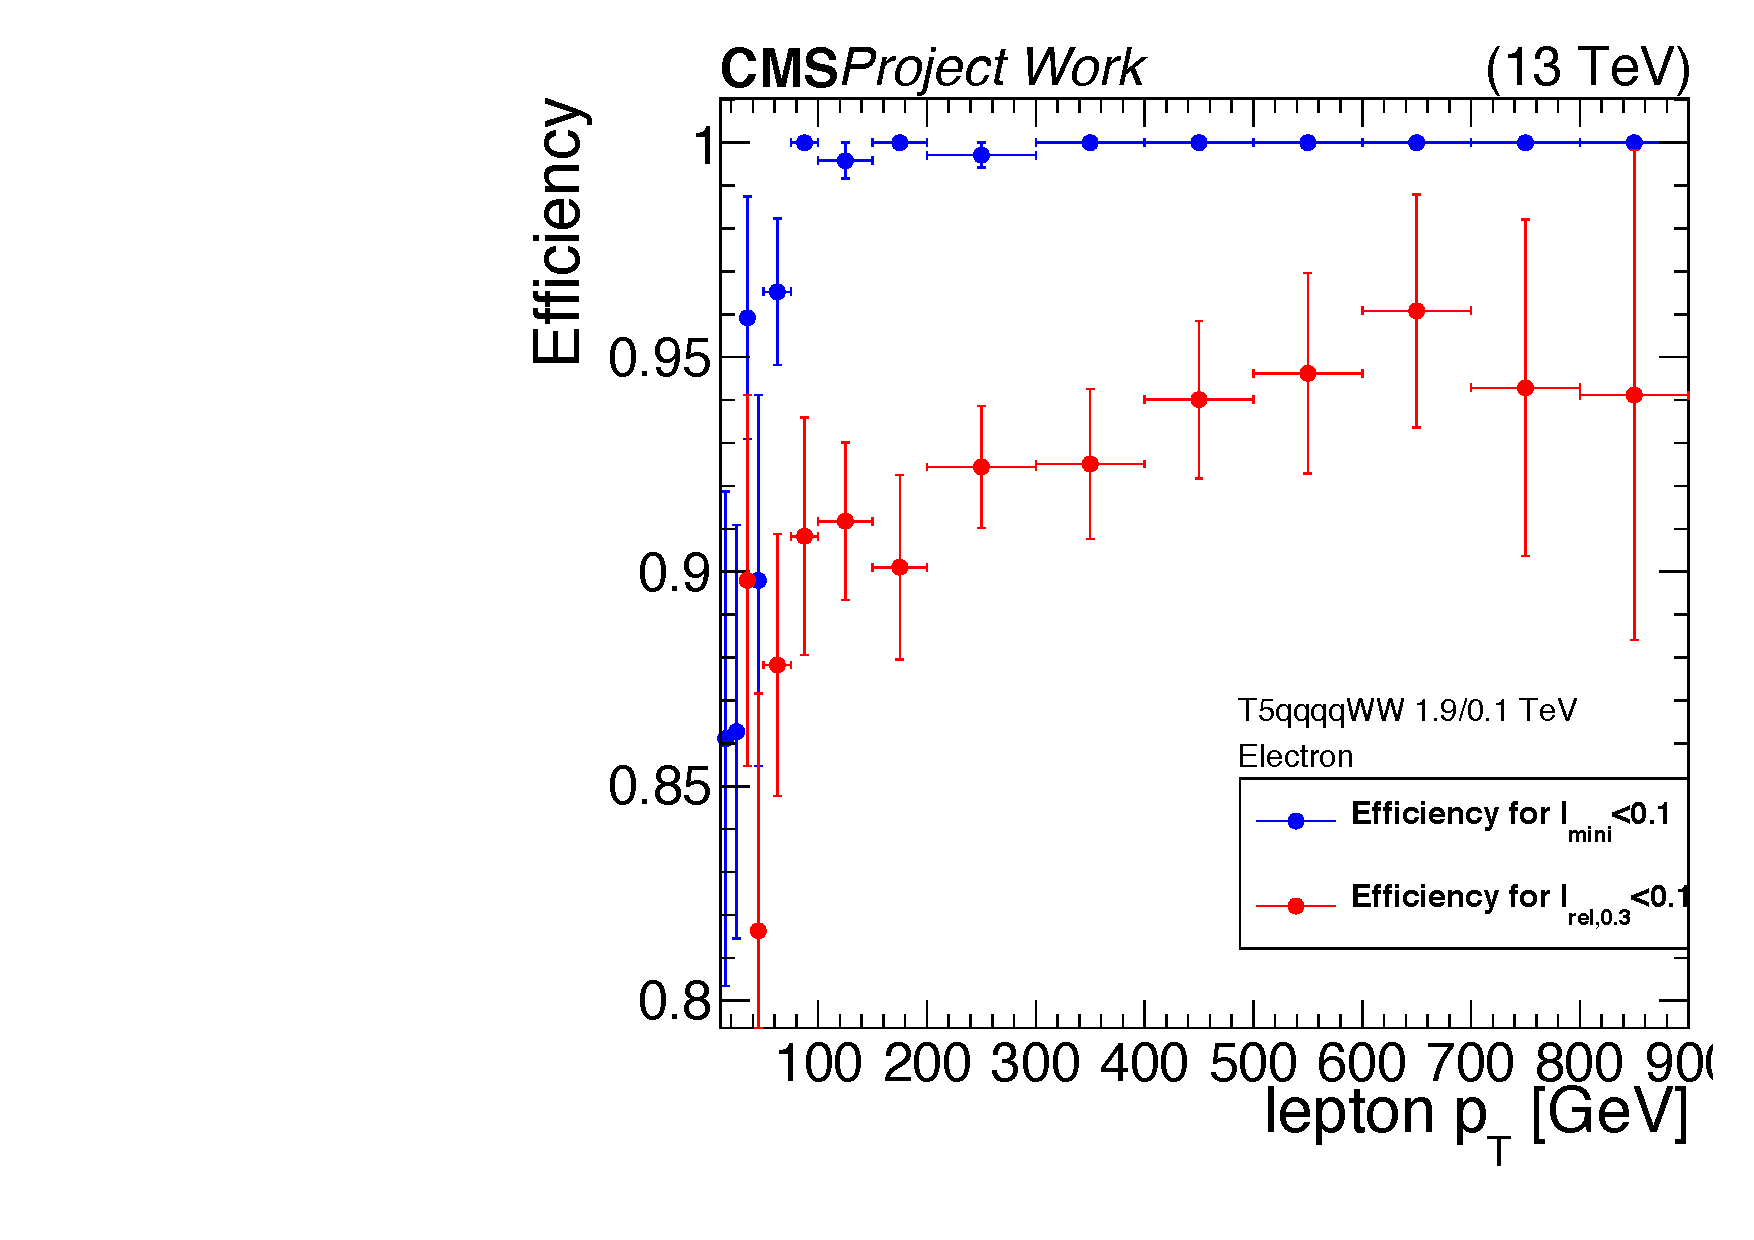
\includegraphics[width=0.45\textwidth]{PhD_Thesis_v4/Plots/lepEff/signal_EleEff.pdf}
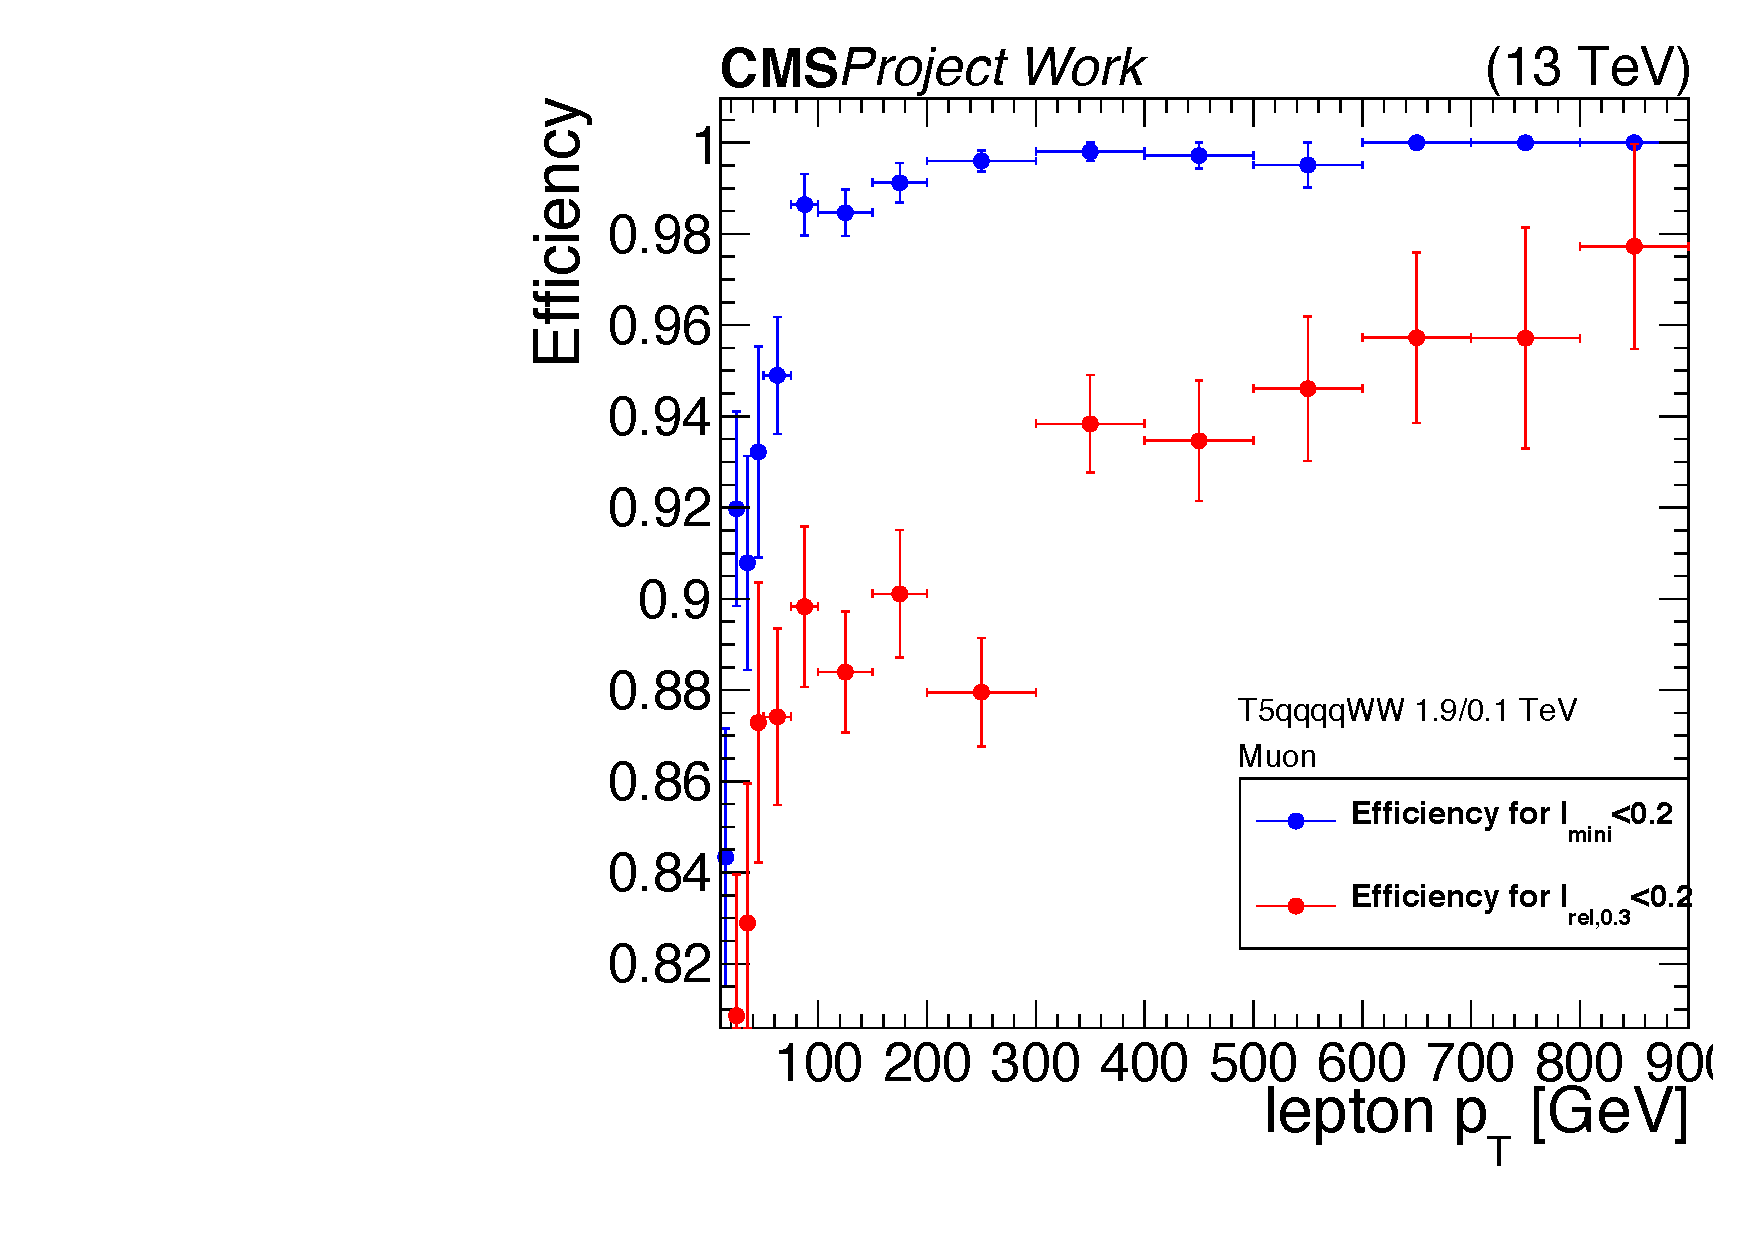
\includegraphics[width=0.45\textwidth]{PhD_Thesis_v4/Plots/lepEff/signal_MuEff.pdf}\\
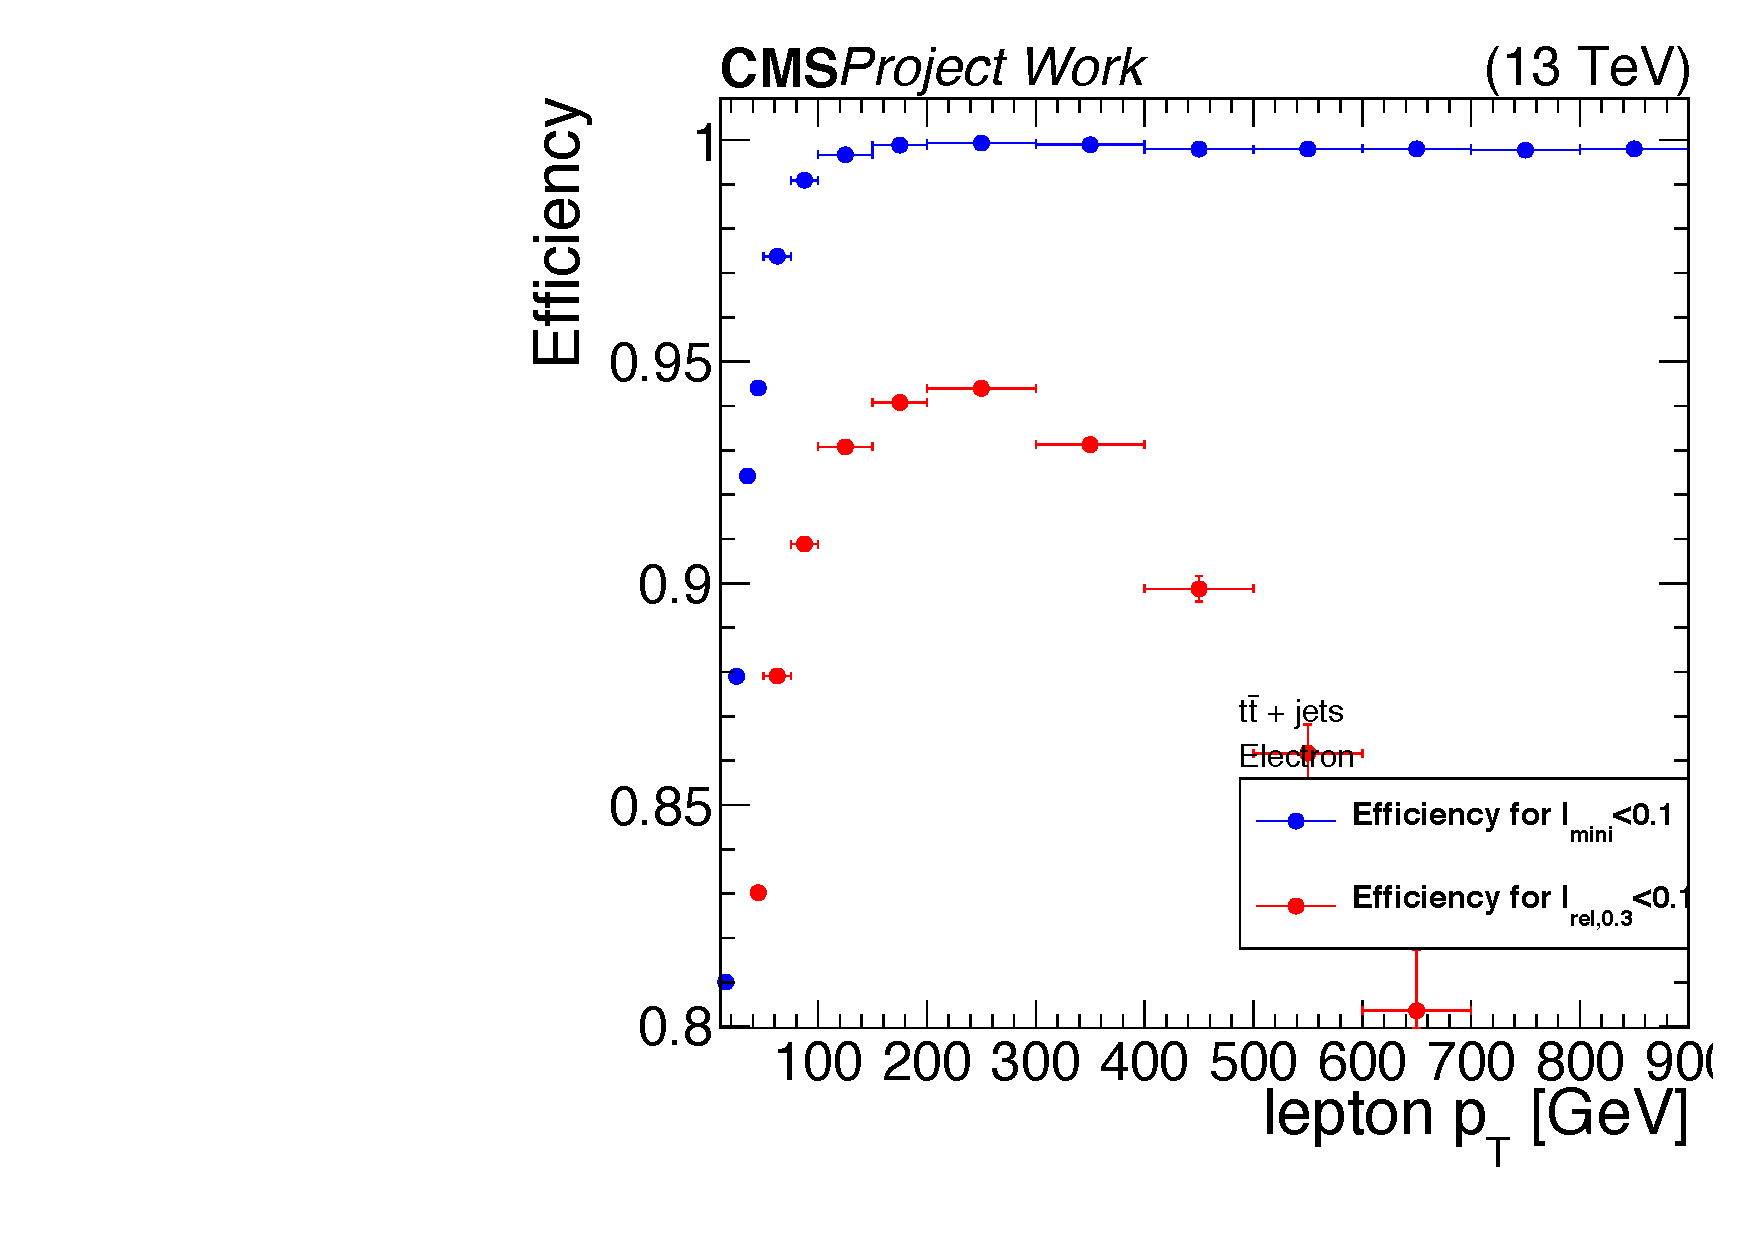
\includegraphics[width=0.45\textwidth]{PhD_Thesis_v4/Plots/lepEff/ttJets_EleEff.pdf}
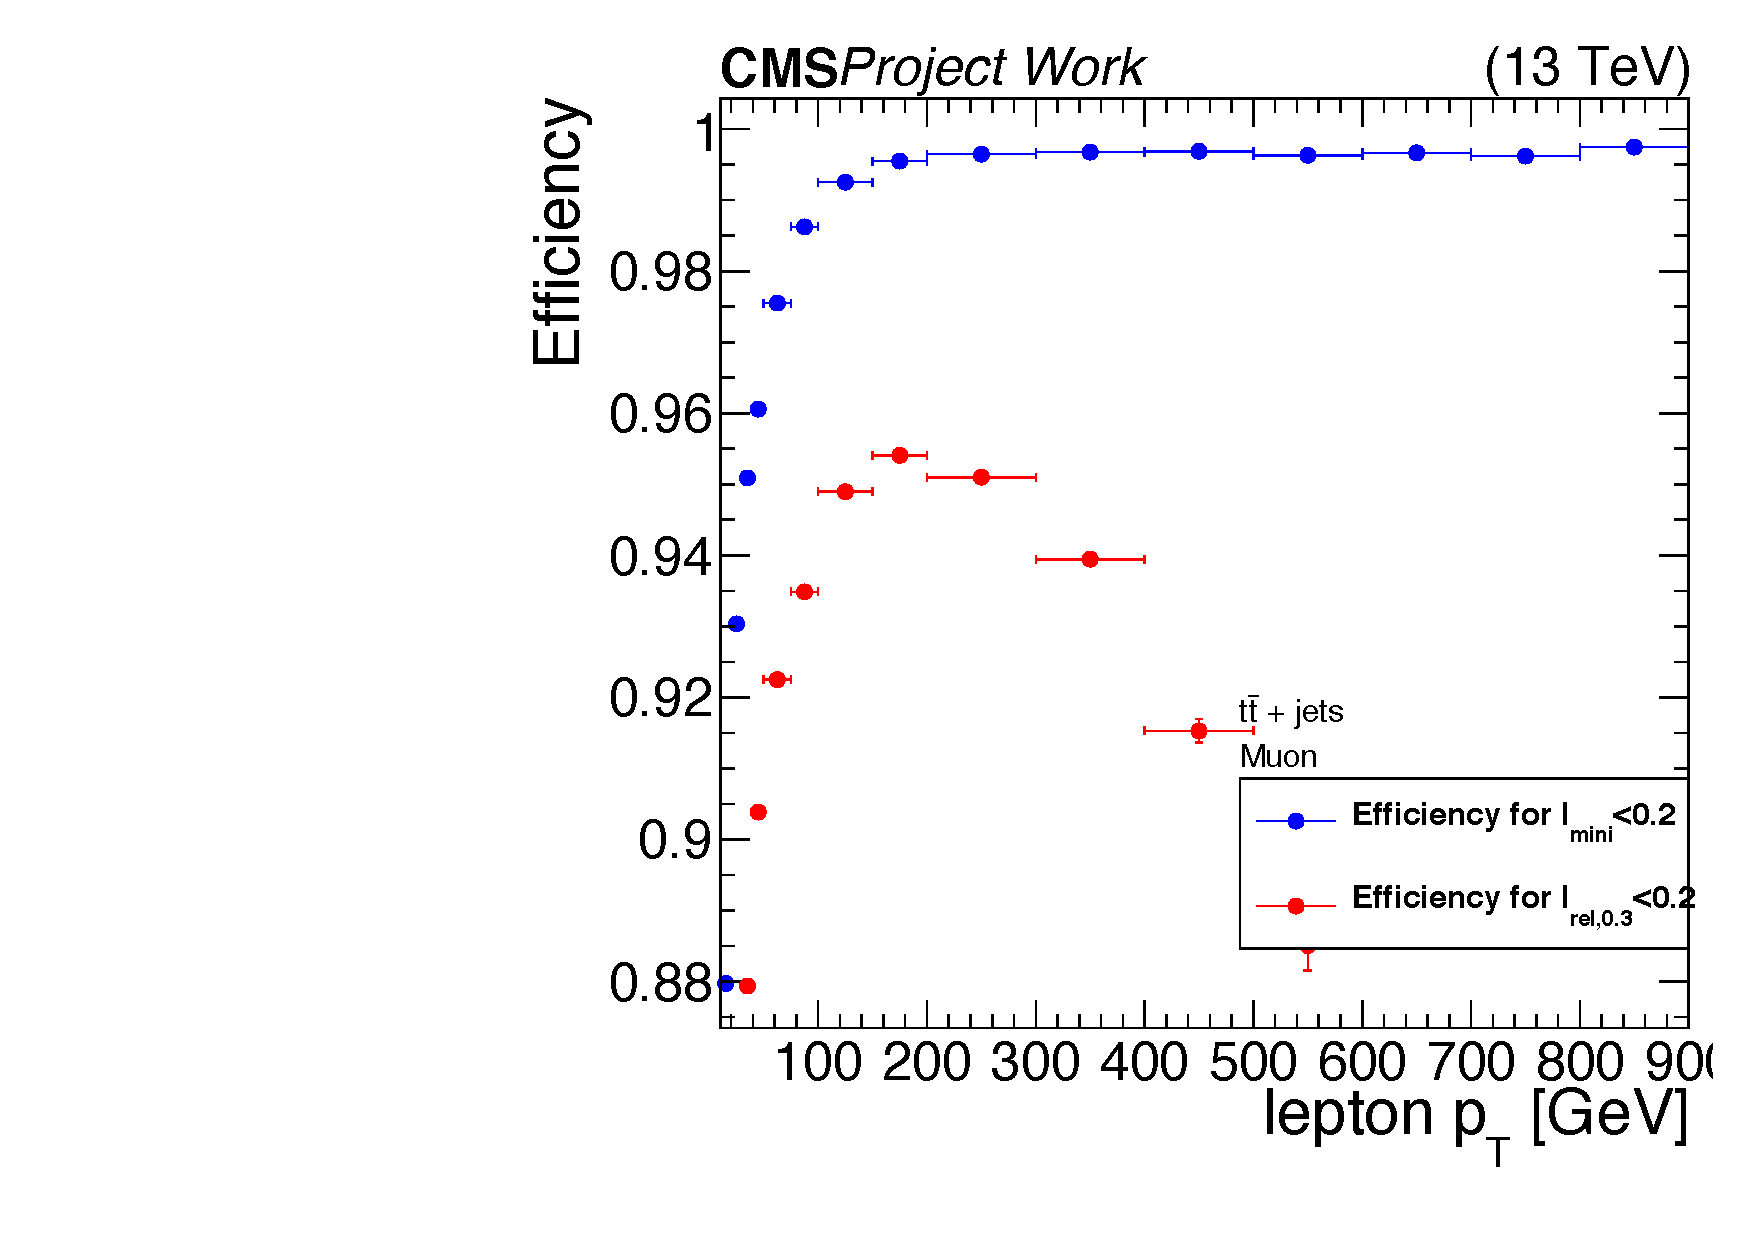
\includegraphics[width=0.45\textwidth]{PhD_Thesis_v4/Plots/lepEff/ttJets_MuEff.pdf}
\caption[Isolation efficiency comparisons]{\label{fig:lep_Eff} Isolation efficiency for simulated events for both of the mini and relative isolation is shown. The upper panel plots show T5qqqqWW (1900,100) model for electrons and muons while the lower panel plots display the efficiency in $\ttJets$ events.}
\end{center}
\end{figure}
%\newpage
\section{Missing transverse energy}
Weakly interacting massive particles, as predicted by the signal models, leave no trace in the CMS detector. Only the imbalance in transverse momentum can indirectly hint towards their existence. Missing transverse momentum~($\METvec$)~\cite{MET} is calculated from the negative transverse vector sum of all PF candidates,
% Therefore, $\METvec$ can be formulated as the negative vector sum of the transverse momentum $\pt$ of all observed particles:
 \begin{eqnarray}
 \label{Eqn:MET}
{\METvec =  -\sum_i\ptveci}\,.
\end{eqnarray}
%Otherwise, the case where $i$ stands for the calorimeter deposits is a another $\MET$ type used in CMS which is known as $Calo-\MET$. A third type of $\MET$ is an improved version of $Calo-\MET$ by corrections obtained from the tracking detector and it is called $TC-\MET$.
The $\MET$ can be mismeasured for several reasons, such as the non linearity of the calorimeter response for hadronic particles, or the minimum energy thresholds in the calorimeters. The bias in the $\MET$ measurement due to the possible reconstruction problems of PF particles can be reduced by correcting $\MET$ by the vectorial difference in the jet momenta that the jet energy corrections account for.
%propagating the jet energy corrections to the $\MET$ calculation. Additionally, $\MET$ can be biased due to pileup interactions. 
%This contribution can be subtracted as:
%\begin{eqnarray}
%{\METvec^{corr} =  %\METvec-\sum_{PU}f(\vec{v})\vec{v}}\,,
%\end{eqnarray}
%where $\vec{v}$ is the vectorial sum $\pt$ of charged particles associated with a given pileup vertex. The factor $f(\vec{v})\vec{v}$ gives the expected total $\METvec$ for each pileup interaction.\\
%Naturally, as it can be understood from the name, $PF-\MET$ is reconstructed by using the particle flow algorithm \cite{MET}. \\
%In the CMS detector, a momentum imbalance can be also originated through the various subdetector malfunctions, reconstruction effects. \\
%To be able to determine the amount of this $fake-\MET$, generally DY events where a Z boson decays to two opposite sign leptons are used because of the fact that in these kind of events the expected $real-\MET$ contribution is very low. In data, these events are selected by requiring the invariant mass of the dimuon or dielectron system is inside the Z-boson mass window, 60GeV$<M_{\ell\ell}<$120GeV.\\
In CMS, particles are produced uniformly in $\phi$, thus $\METvec$ is expected to have a flat distribution in $\phi$. However, due to the $\phi$-dependence of the detector response, imperfect alignment of different detector subsystems, and a $\sim4$~mm shift between the centre of the detector and beamline~\cite{CMS-PAS-TRK-10-003}, an asymmetry in $\phi$ is observed in data and in simulated events.\\
The observed $\phi$-asymmetry can also be viewed as a mean shift in the $\METvec$ components along the x and y detector axes. The shift shows an increasing trend in shape of a second order polynomial as a function of $\sum \pt$ of the PF candidates. To obtain the corrections, this correlation is used. First, polynomial fits are performed on $\mex$ and $\mey$ distributions as a function of $\sum \pt$ of PF candidates in various $\eta$ bins. Examples of these fits are shown in Fig. \ref{fig:phiFits}, where the dependence of $\langle\mex\rangle$ and $\langle\mey\rangle$ 
on multiplicity of PF candidates can be formulated as:
\begin{eqnarray}
\left<\mex \right> & = & c_{x_o} \cdot x + c_{x_s} \cdot x^2, \nonumber \\
\left<\mey \right> & = & c_{y_o} \cdot x + c_{y_s} \cdot x^2.
\label{eq:metPhiAsymmetryFitModel}
\end{eqnarray}
\begin{figure}[!h]
\begin{center}
\subfigure[$\mex$, sum $\pt$ of gamma in minus endcap region]{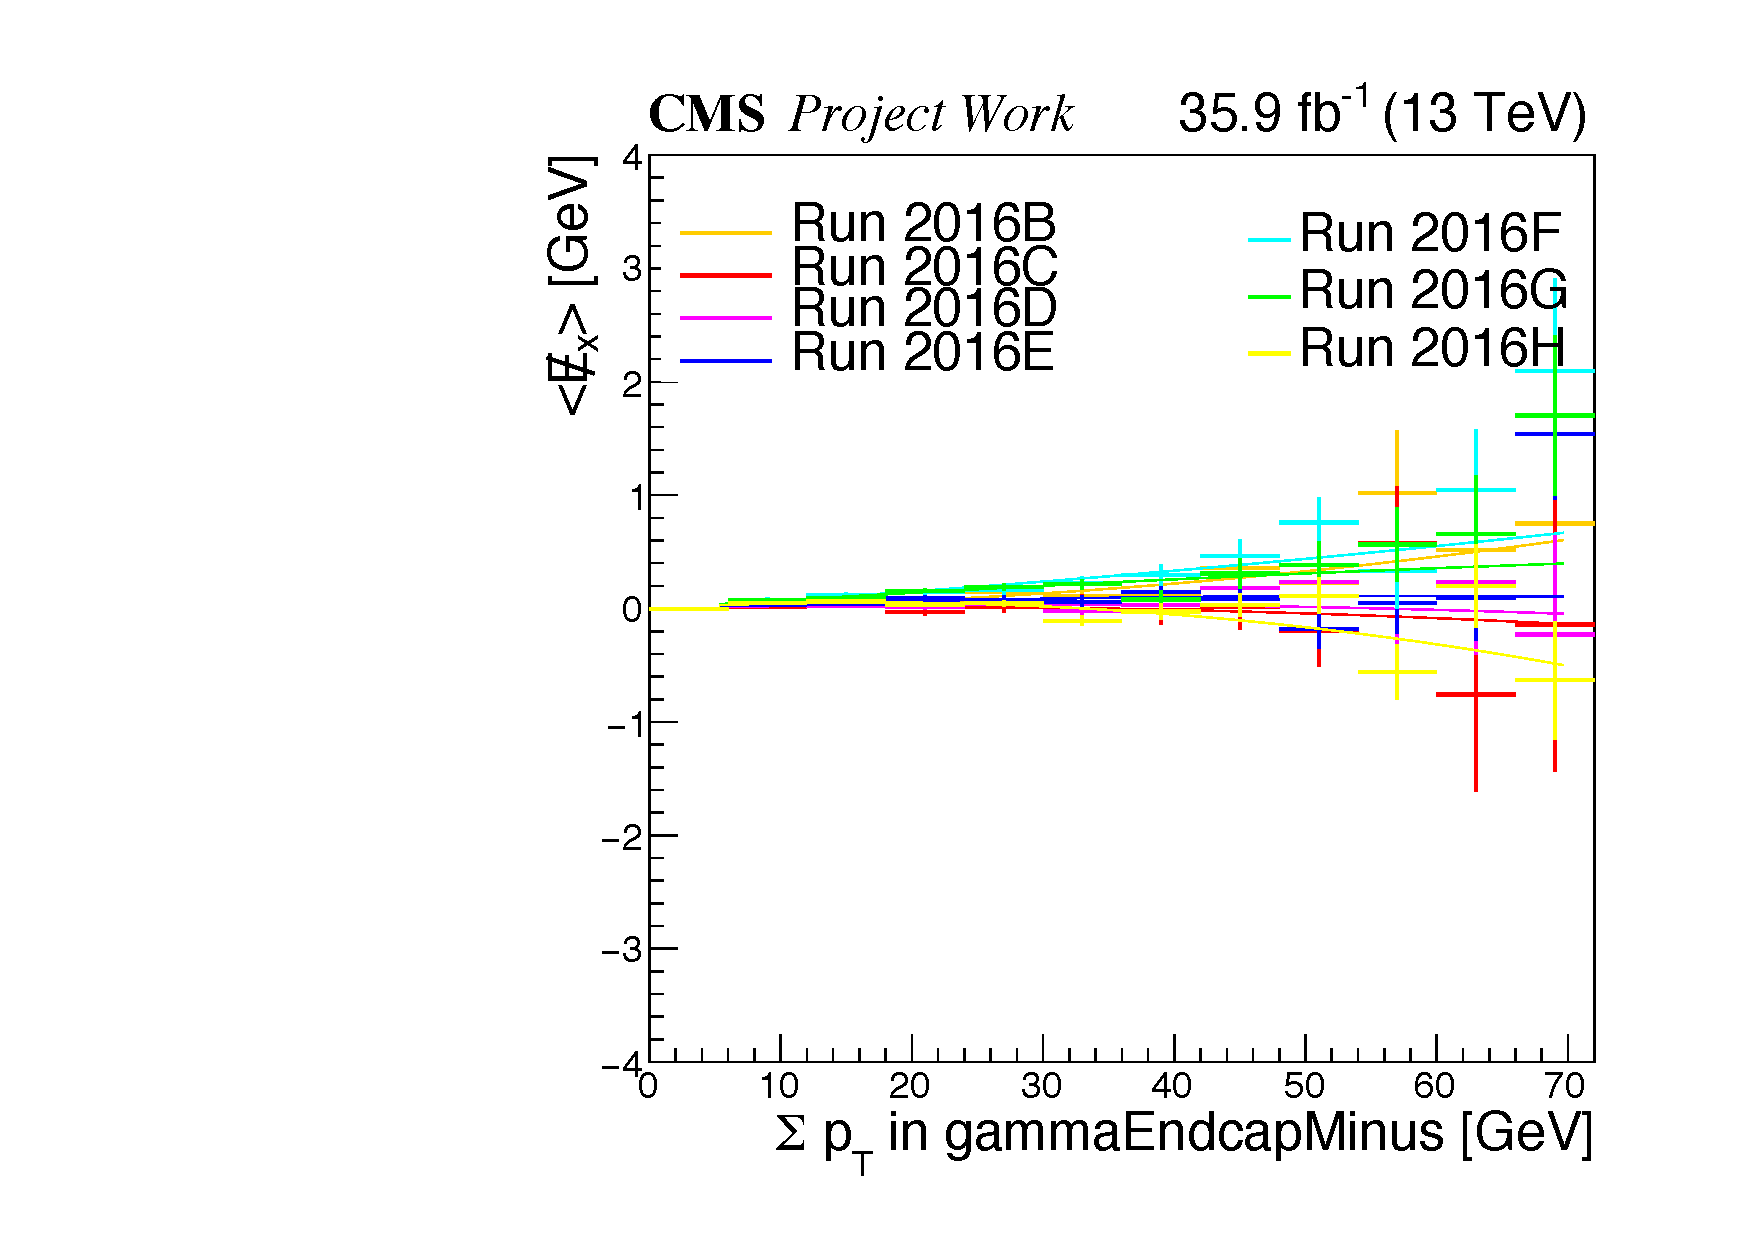
\includegraphics[width=0.45 \textwidth]{PhD_Thesis_v4/Plots/metphi/gammaEndcapMinus_Px_sumPt_.pdf}}
\subfigure[$\mey$, sum $\pt$ of gamma in minus endcap region]{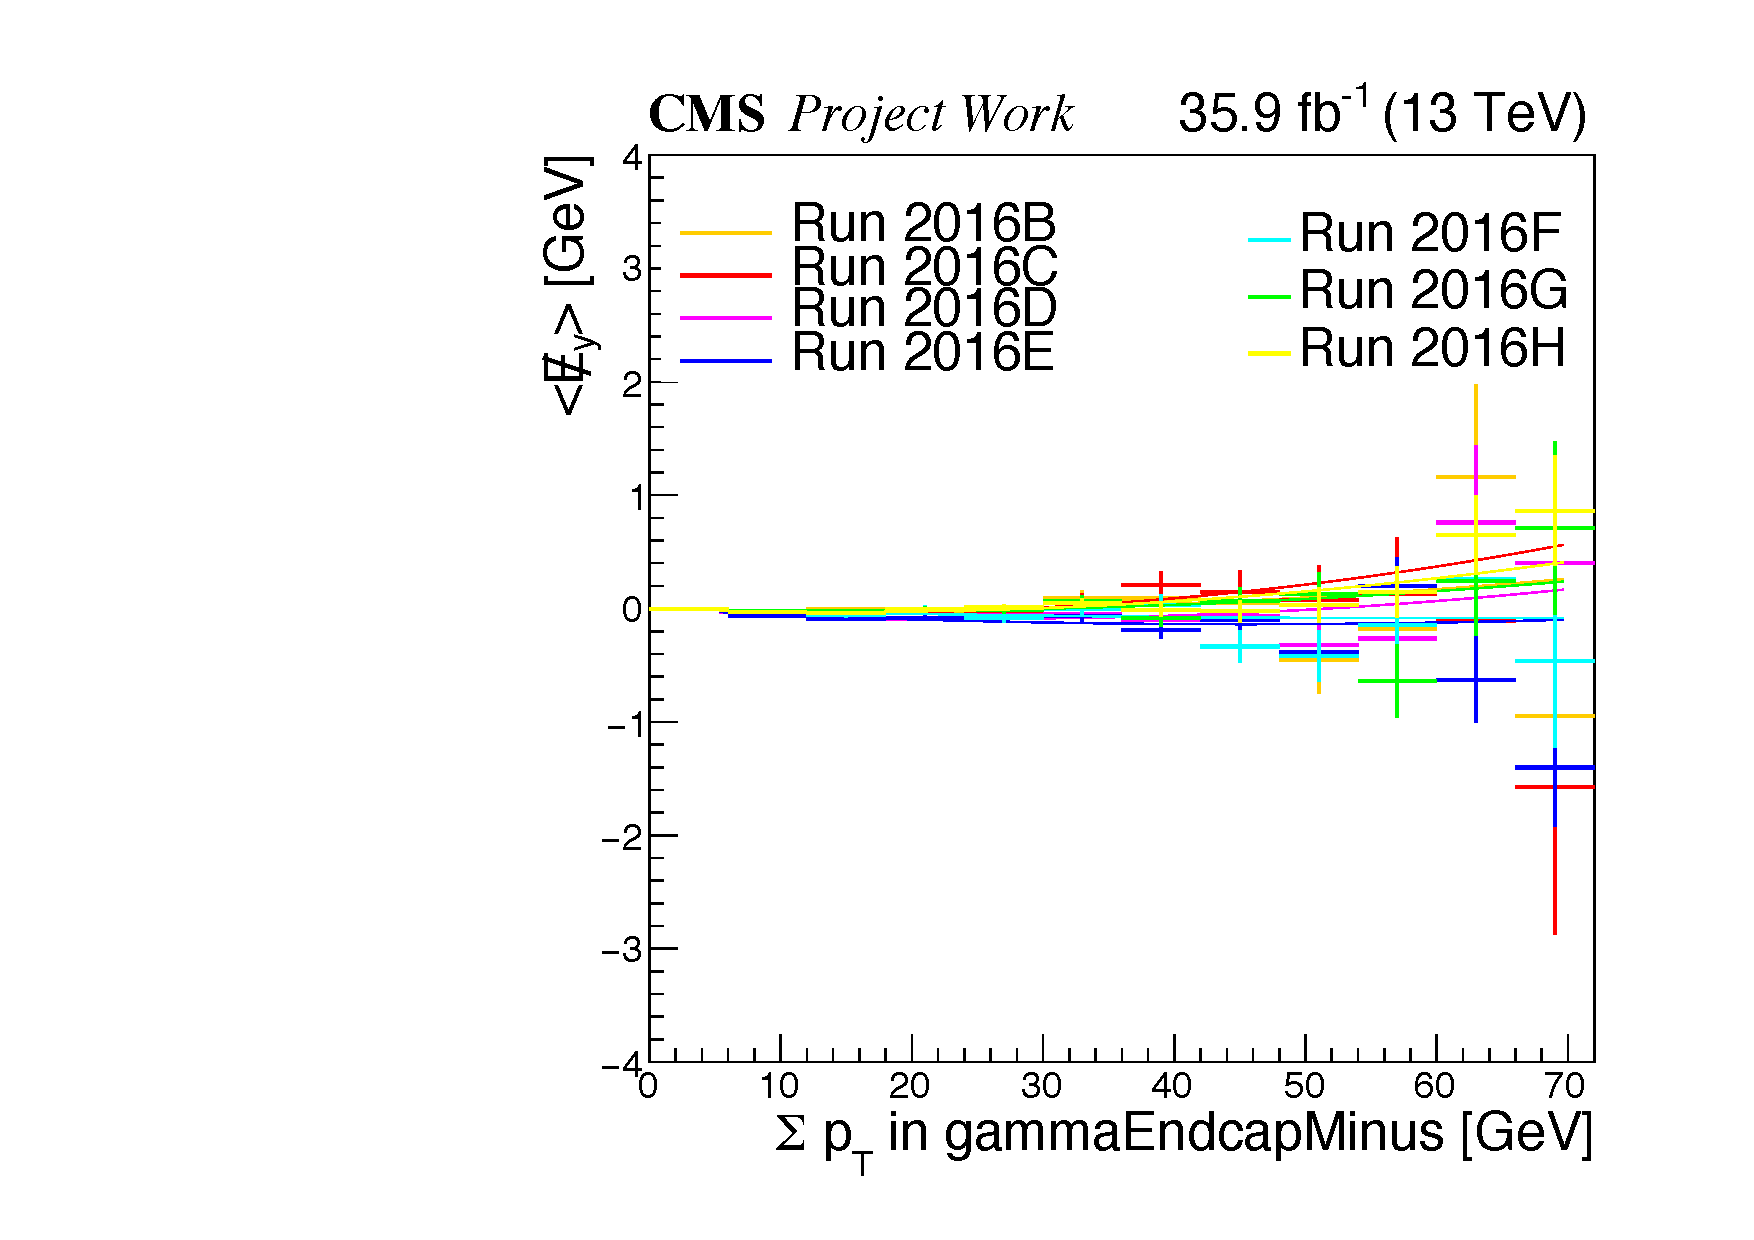
\includegraphics[width=0.45 \textwidth]{PhD_Thesis_v4/Plots/metphi/gammaEndcapMinus_Py_sumPt_.pdf}} \\
\subfigure[$\mex$, sum $\pt$ of neutral hadrons in barrel region]{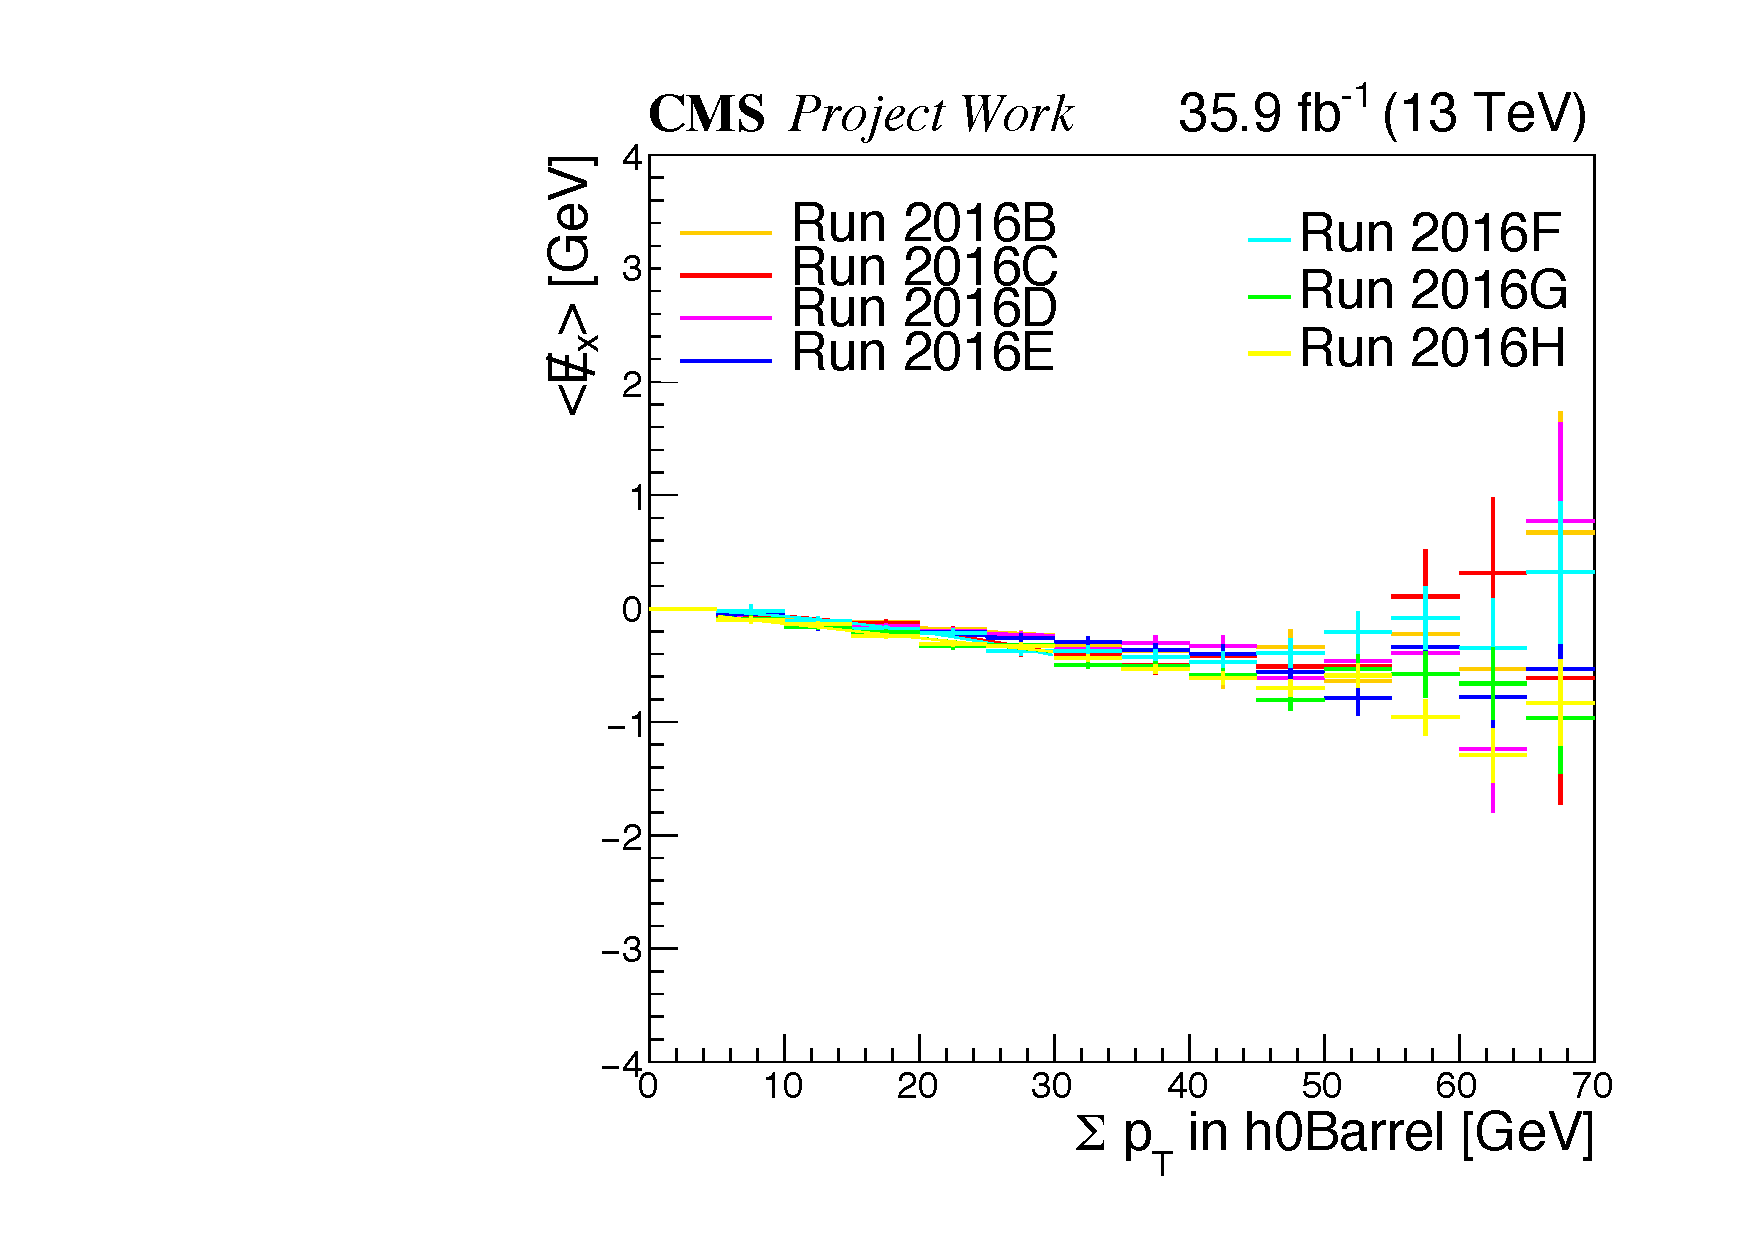
\includegraphics[width=0.45 \textwidth]{PhD_Thesis_v4/Plots/metphi/h0Barrel_Px_sumPt_.pdf}}
\subfigure[$\mey$, sum $\pt$ of neutral hadrons  in barrel region]{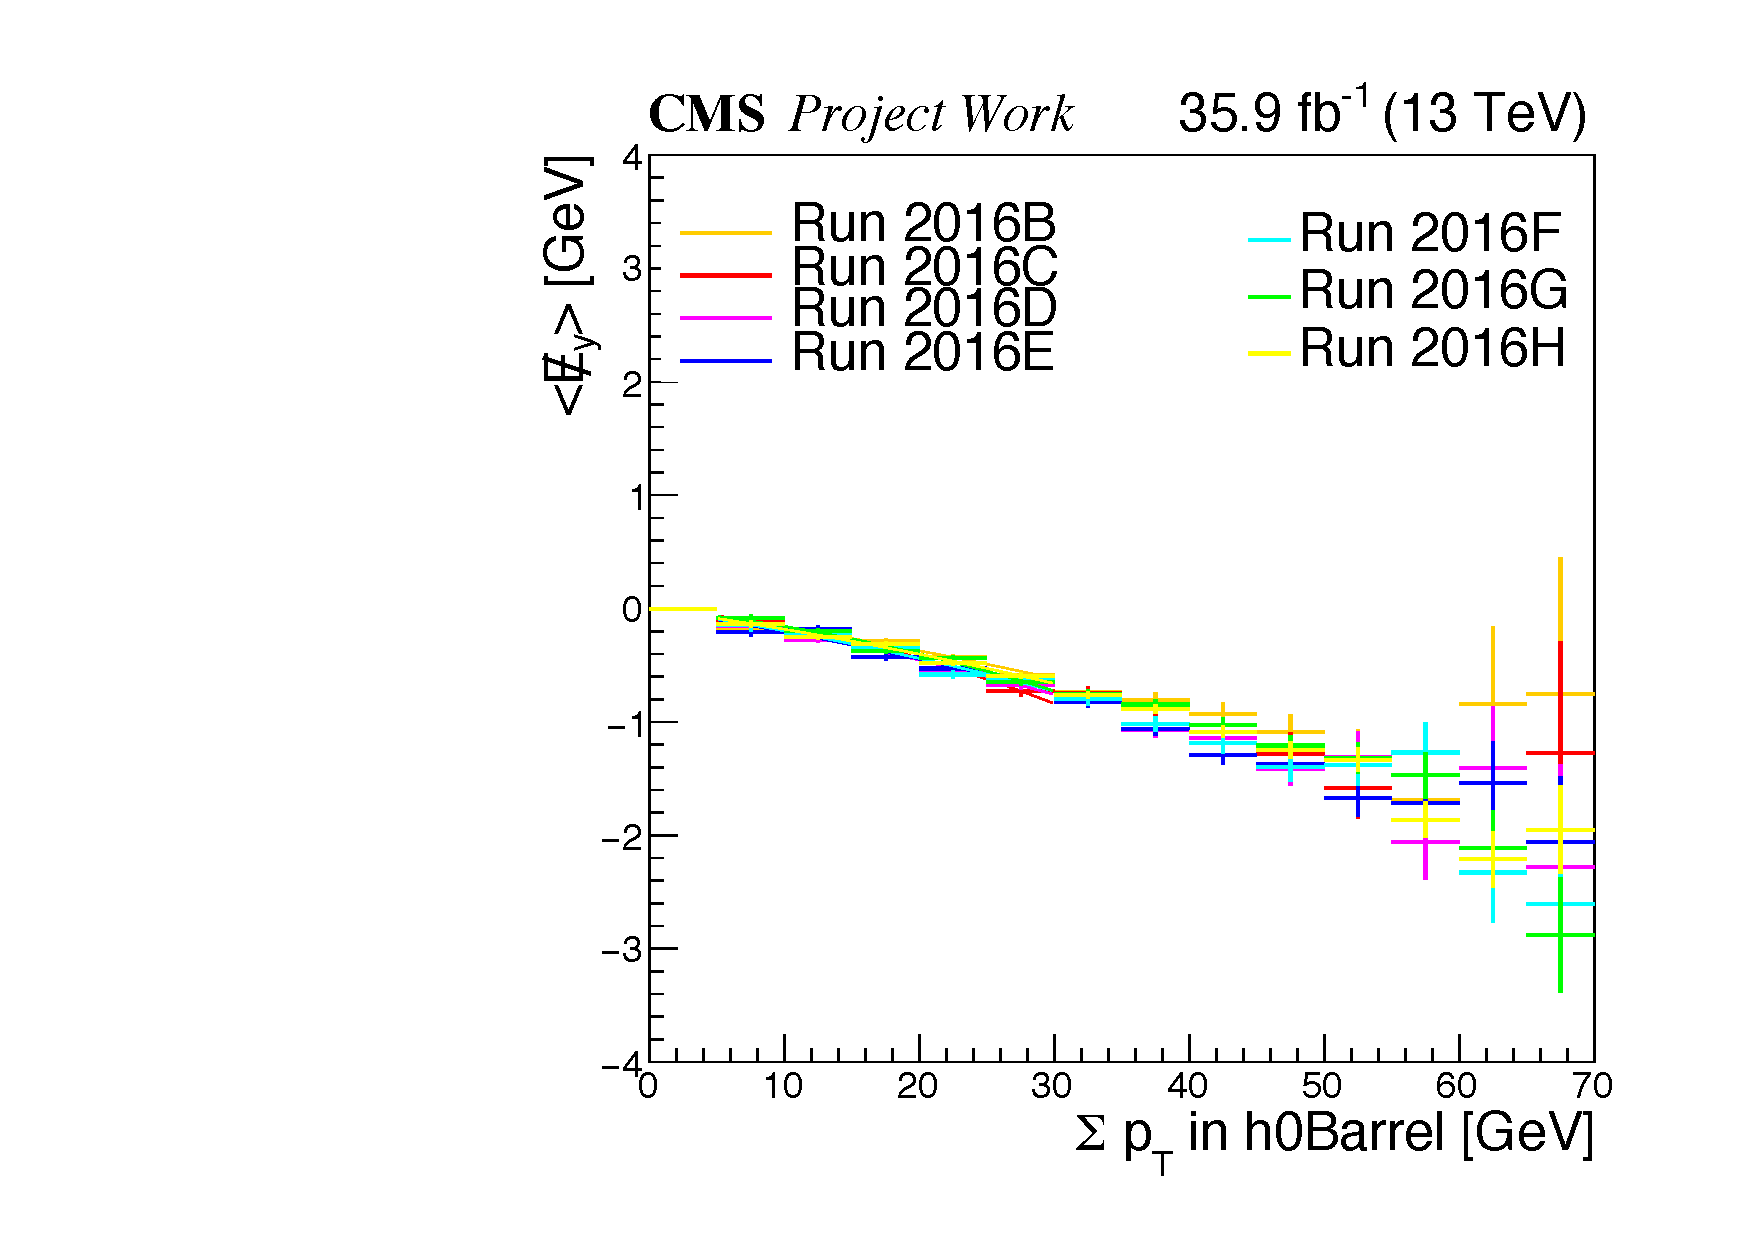
\includegraphics[width=0.45 \textwidth]{PhD_Thesis_v4/Plots/metphi/h0Barrel_Py_sumPt_.pdf}} \\
\caption{
  PF candidate multiplicity fits for \mex and \mey in different $\eta$ regions. Different colored lines represent different data taking run ranges. The Y-axis shows the average value of the x- and y-components of missing energy while X is the sum $\pt$ of the corresponding PF candidate.
  }\label{fig:phiFits}
\end{center}
\end{figure}
After the fits are performed, the corrected $\mex$ and $\mey$ can be obtained on an event-by-event basis as:
\begin{eqnarray}
\mex^\mathrm{corr} &=&  \mex - \left<\mex \right>= \mex  -(c_{x_o} \cdot x + c_{x_s} \cdot x^2), \nonumber \\
\mey^\mathrm{corr} &=&  \mey - \left<\mey \right> = \mey -(c_{y_o} \cdot x + c_{y_s} \cdot x^2).
\end{eqnarray}
The coefficients $c_{x_0}$, $c_{x_s}$, $c_{y_0}$, and $c_{y_s}$ are determined
separately from data and simulated samples. In data, the corrections are obtained in dimuon events with the invariant mass of the dimuon system is inside the Z-boson mass window, 60GeV$<M_{\ell\ell}<$120GeV. In simulated samples, the corrections are obtained by using DY events where a $Z$ boson decays to two opposite charged leptons. In such events the expected ${\rm genuine-}\MET$ contribution is very low, thus they provide a very good environment to measure $\MET$ mismodelings. The validation of the procedure is performed by using $\ttJets$ and $\wJets$ simulated samples. 
Figure~\ref{fig:metphiCorr} shows $\MET$ before and after the correction for simulated events. It is evident that there is no significant change to the spectrum while $\MET_{\phi}$ is properly corrected.
\begin{figure}[!h]
\begin{center}
\subfigure[$\MET\,\,\phi$]{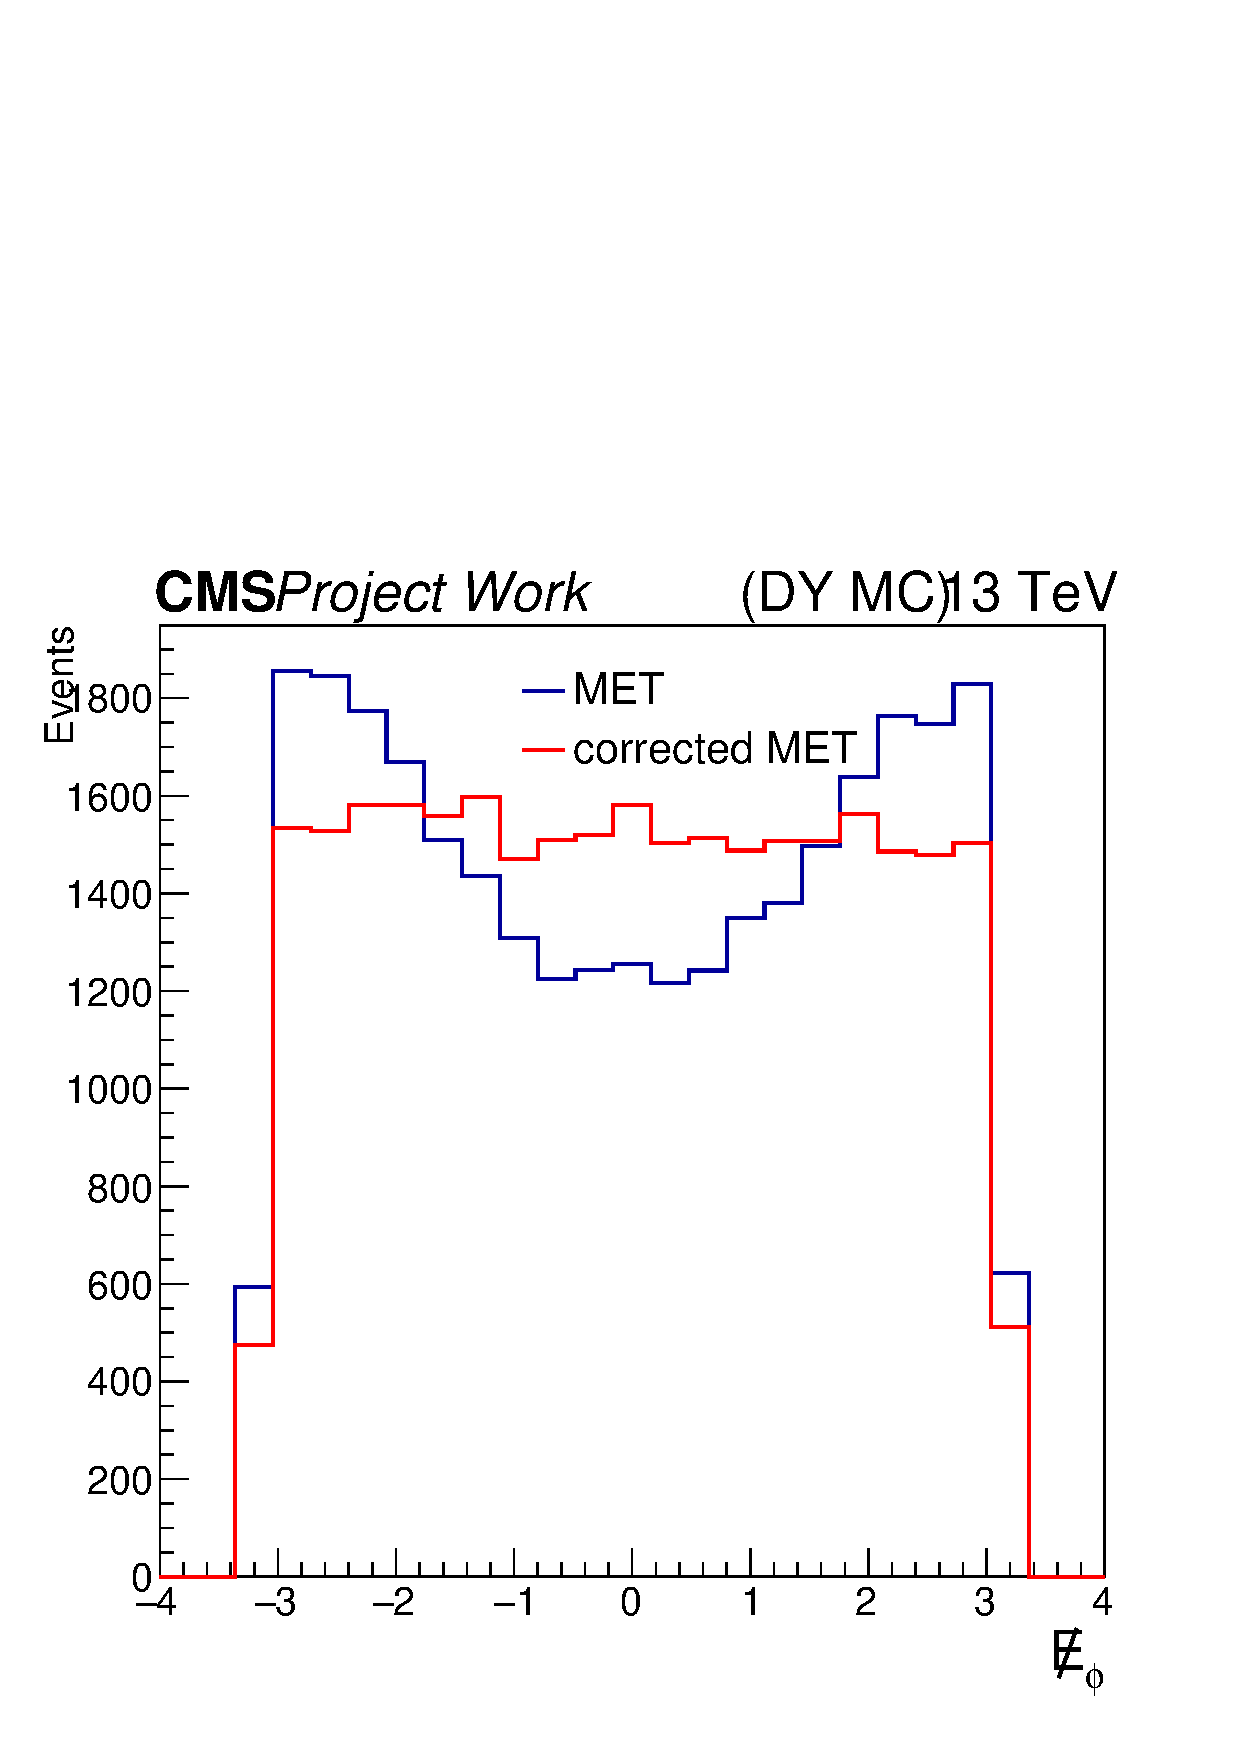
\includegraphics[width=0.5\textwidth]{PhD_Thesis_v4/Plots/metphi/DY_Comp_For_thesis.pdf}}
\subfigure[$\MET\,\,\pt$]{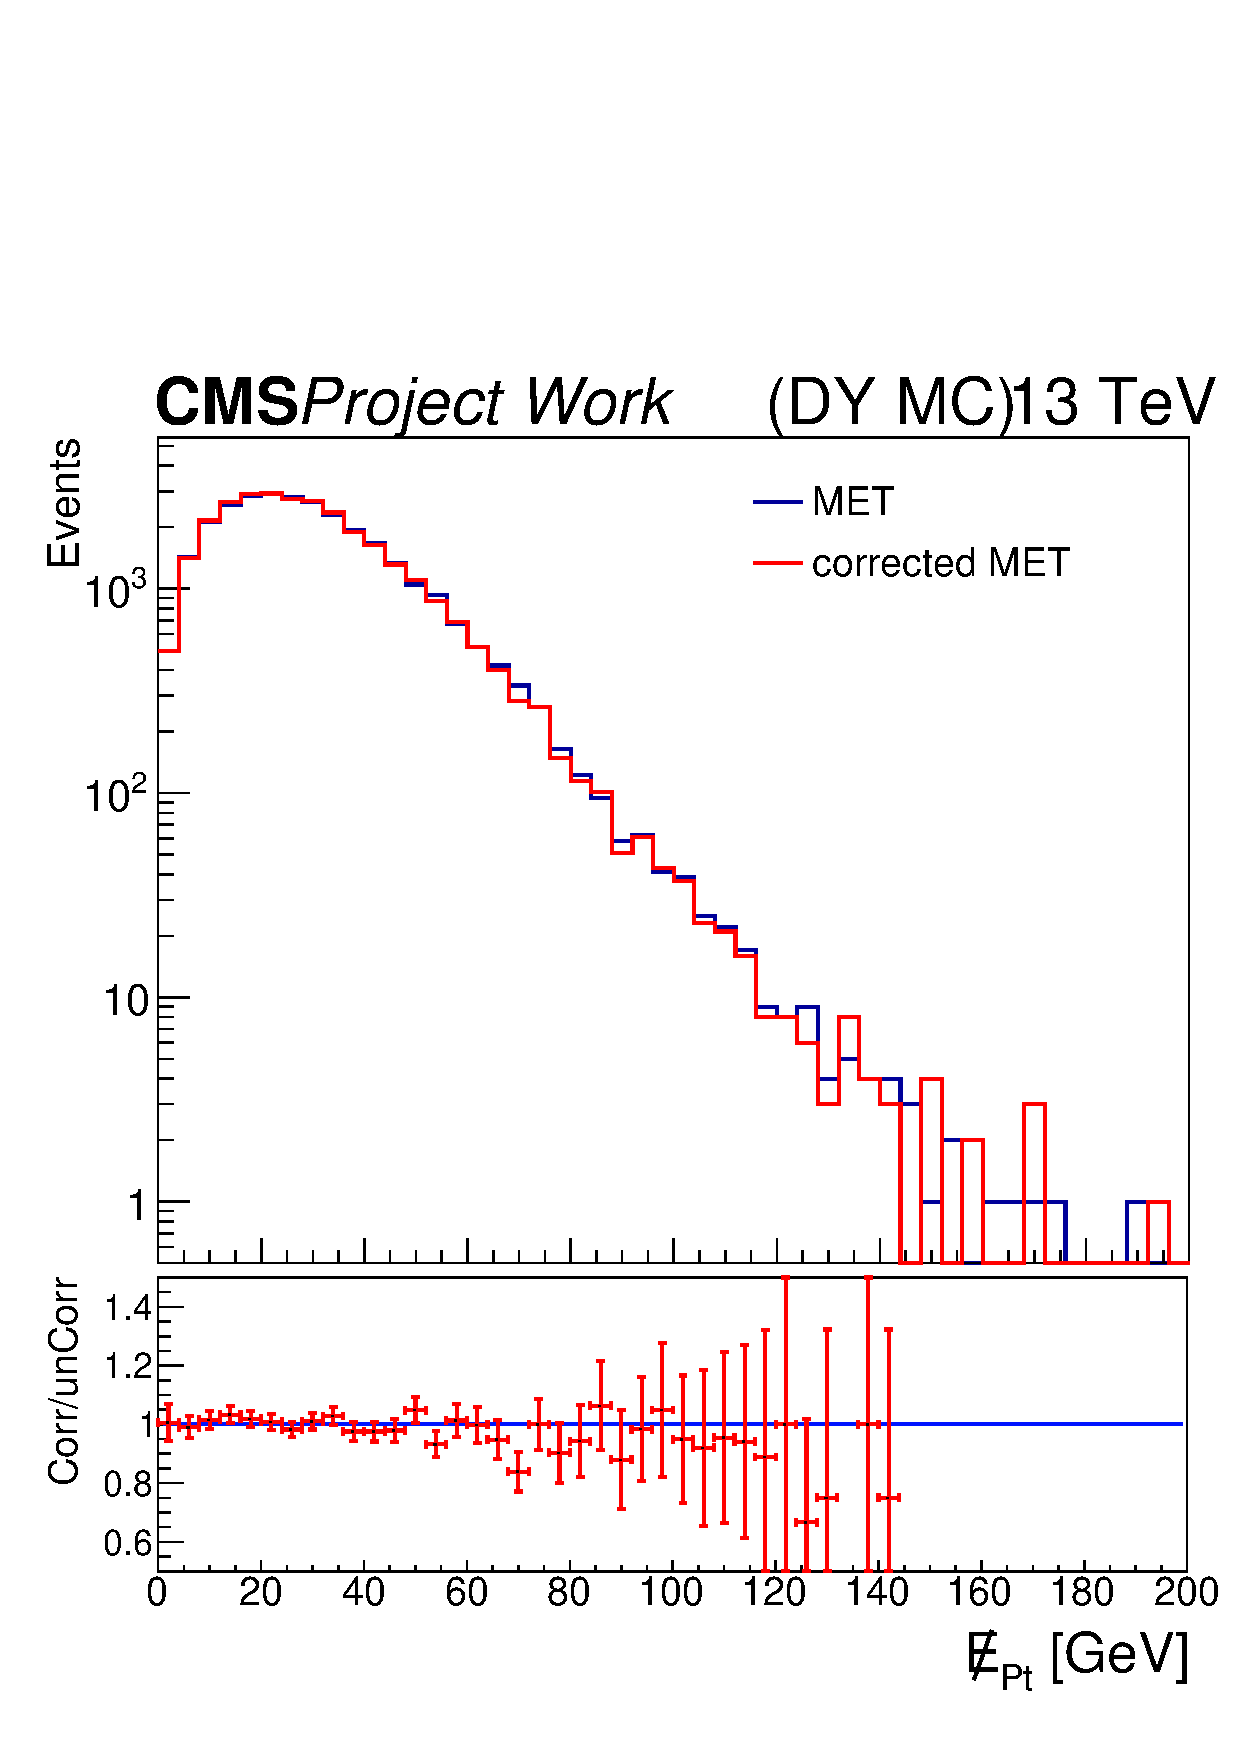
\includegraphics[width=0.45\textwidth]{PhD_Thesis_v4/Plots/metphi/DY_Comp_PT_For_thesis.pdf}}\\
\caption{
  $\MET$ $\phi$(left) and $\pt$(right) distributions before(blue) and after(red) corrections in simulated Drell-Yan events.  
  }\label{fig:metphiCorr}
\end{center}
\end{figure}
%\newpage
